\documentclass{beamer}
\setbeameroption{show notes}
%\setbeameroption{show only notes}
%\setbeameroption{show notes on second screen} % My version of beamer must be too old for this option...
\usetheme{PaloAlto}

\usepackage{fontspec}
\setsansfont{Arial Unicode MS}

\usepackage{listings}
\usepackage{expex}
\resetcountonoverlays{excnt} % Needed so that ExPex example numbers aren't incremented on each overlay (see http://tex.stackexchange.com/questions/162646/example-numbering-changes-between-overlays)
\usepackage{verbatim}
\usepackage{url}
\usepackage{latexsym}
\usepackage{graphicx}


\usepackage{pgf}
\usepackage{tikz}
\usetikzlibrary{shapes,shapes.geometric,arrows,fit,calc,positioning,decorations.markings}



% My Package Includes
\usepackage{upquote} % For real apostrophes (see http://tex.stackexchange.com/questions/63345/how-to-make-a-real-apostrophe-or-single-quote-in-latex#63348)
\usepackage{comment}
\usepackage{xcolor}
\definecolor{dark-blue}{rgb}{0.15,0.15,0.7}
\usepackage{hyperref}
%\hypersetup{colorlinks, linkcolor={dark-blue}, citecolor={dark-blue}, urlcolor={dark-blue}}
\hypersetup{colorlinks, linkcolor=black, citecolor=black, urlcolor=black}
\usepackage{booktabs}
\frenchspacing % Normal (single) spaces after periods.  Cf. http://www.read.seas.harvard.edu/~kohler/latex.html
%\usepackage{natbib}
\usepackage[shortcuts]{extdash} % use "\-/" to help LaTeX insert hyphen/pagebreaks
\usepackage[textwidth=0.9in]{todonotes}
\newcommand{\smalltodo}[2][]
    {\todo[caption={#2}, #1]
    {\tiny#2\normalsize}}


\newtheorem{requirement}{Requirement}

\setbeamertemplate{theorem begin}{{
\inserttheoremheadfont
\inserttheoremname
\inserttheoremnumber
\ifx\inserttheoremaddition\@empty\else\ \inserttheoremaddition \fi%
\inserttheorempunctuation
}}
\setbeamertemplate{theorem end}{}

\begin{document}



\title[LingSync \& OLD] % (optional, use only with long paper titles)
{LingSync \& the Online Linguistic Database}
%ენატს


\author[~]{Joel Dunham \inst{1} \and Gina Chiodo \inst{2} \and Josh Horner \inst{3}}
\institute[UBC, LingSync.org]{\inst{1} University of British Columbia \and %
                      \inst{2} iLanguage Lab \and %
                      \inst{3} Amilia}


                      \subtitle
                      {New models for the collection and management of data for language communities, linguists and
                      language learners}

\date[ComputEL 2014] % (optional, should be abbreviation of conference name)
{ComputEL Workshop, June 26 2014\\52nd Annual Meeting of the Association for Computational Linguistics (ACL) }



% \AtBeginSubsection[]
% {
% \setbeamertemplate{sidebar left}{}
%   \begin{frame}<beamer>
%     \frametitle{Outline}
%     \tableofcontents[currentsection,currentsubsection]
%   \end{frame}
%   \setbeamertemplate{sidebar left}[sidebar theme]
%
% }

\setbeamertemplate{sidebar left}{}
\begin{frame}
\titlepage
\note{Hello everyone. My name is Joel and this is Gina.}
\note[item]{We are here to talk to you today about LingSync and the
Online Linguistic Database.}
\note[item]{These are free non-proprietary open source tools that facilitate collaborative 
fieldwork on endangered languages.}
\note[item]{This presentation will provide a very high overview of the systems for a mixed audience.}
\note[item]{However, we are at a transition point since we are beginning to
    merge these two tools under the LingSync name. We're very excited to be here
    to be part of the discussion about how mobile or web technologies and
    computational linguistic advances can benefit fieldwork on endangered
    languages.}
\end{frame}
\setbeamertemplate{sidebar left}[sidebar theme]


%%%%%%%%%%%%%%%%%%%%%%%%%%%%%%%%%%%%%%%%%%%%%%%%%%%%%%%%%%%%%%%%%%%%%%%%%%%%%%%%
% BACKGROUND
%%%%%%%%%%%%%%%%%%%%%%%%%%%%%%%%%%%%%%%%%%%%%%%%%%%%%%%%%%%%%%%%%%%%%%%%%%%%%%%%

\section{Background}


% FIELDWORK
%%%%%%%%%%%%%%%%%%%%%%%%%%%%%%%%%%%%%%%%%%%%%%%%%%%%%%%%%%%%%%%%%%%%%%%%%%%%%%%%

\subsection[Fieldwork]{Endangered languages fieldwork}\label{sec:fieldwork}


% CONTEXT
%===============================================================================

\begin{frame}
\frametitle{Context}
\begin{itemize}
    \item Context of rapid language loss (Harrison 2007, Krauss 1992)
    \item Language diversity and vitality are valuable scientifically,
        culturally, and socially (Hallett et al. 2007)
    \item Computational approaches and formalisms can benefit fieldwork
        (Bird 2009) % TODO which paper is this, can we clarify if its computational tools, new technologies or computational linguistics?
    %\item Important differences (Crippen \& Robinson 2013)
\end{itemize}
\note[item]{So, it hardly needs to be stated that we are in a situation where
    a significant portion of the world's languages are predicted to be extinct
    or "sleeping" in the very near future.}
\note[item]{For those who might be skeptical of a strong link
    between social well-being and language vitality Hallett et al. (2007) 
     describes a study which finds a
    correlation between higher levels of Aboriginal language use in British
    Columbia First Nations bands and lower youth suicide rates.}
\note[item]{And clearly we're all here because we think that computational
    linguistics can contribute to the
    documentation, study, and/or revitalization of endangered languages
     if such a collaboration can be facilitated.}

\end{frame}


% DEBATES
%===============================================================================

\begin{frame}
\frametitle{Debates}
\begin{itemize}
    \item<1-> How to balance our limited time resources?
        \note[item]<1>{There are a number of ongoing debates.}
        \note[item]<1>{First,  how we should
            balance our time given the urgent problem of language endangerment.}
        \begin{itemize}
            \item<2->Less descriptive artifacts, more aligned speech recording, more grass-roots 
                community involvement can revitalize the language (Woodbury 2003, Bird et al. 2014) %TODO we need these references. do they really say less description  I thought Bird said we should do grammars, could we say less analysis to be more precise about the difference of IGT vs grammar modeling?
                \note[item]<2>{Some argue that we could use the majority of our time for  
                     recording speech, re-speakings, and translations, and for
                    generating artifacts for the future.}
                \item<3->Better descriptive artifacts can prevent “data graveyards”
                    (Gippert et al. 2006, cf. Beale 2014)
                \note[item]<3>{Others argue that we can use advances in computational
                    linguistics to expedite language description and
                    analysis.}
            \item<4->In-depth theoretical analysis can uncover previously
                unknown generalizations which can make the community proud to speak their unique language (Murray 2014)
                \note[item]<4>{There is a related debate between typologists and theoretical linguists
                    about how targeted data is elicited, including using translation from the metalanguage
                    and the gathering of grammaticality judgments--- Murray argues, convincingly
                    in my estimation, that hypothesis-driven fieldwork %you know, typologists and descriptive linguists are hypothesis driven too. this is very patronizing.
                    involving the elicitation of negative data can lead to the
                    discovery of significant generalizations that, under a
                    purely framework independant descriptive approach, would remain hidden.}
        \end{itemize}
    \item<5->A duty to collaborate?
        \note[item]<5>{A related debate asks whether the various types of fieldworkers have a duty to collaborate.}
        \begin{itemize}
            \item<6->Language revitalization is paramount; collaboration is imperative (Gerdts 2010)
                \note[item]<6>{At one extreme lies the view that the time overhead which collaboration entails is necessary despite the loss of academically publishable results of fieldwork.}
            \item<7->Collaboration is not always desired (Crippen \& Robinson 2013) %TODO we need this paper, what do they say? do they really call it "lone wolf" and unethical in the same sentence?!
                \note[item]<7>{Others point out that, for a variety of reasons,
                    collaboration is not always possible. The contexts of language
                    endangerment are themselves diverse. Not all communities are 
                    commited to documentation or revitalization. Not all
                    communities need or desire the help of academic fieldworkers. In some
                    cases, the political landscape of an endangered language
                    community is just too complex for a field linguist to navigate. In 
                    these types of situations, the best course of action for all parties
                    involved may be for linguist fieldworkers to respectfully
                    and ethically pursue their own research program.}
        \end{itemize}
    \item<8->Whatever we decide, let's maximize openness, transparency, access, sharing and reuse
        of both data and functionality
        \note[item]<8>{These are complex and relevant issues. However, to a certain
            extent the LingSync/OLD approach can sidestep them. The attitude we advocate
            is something along the lines of "can't we all just get along?". We want to
            help contribute towards an infrastructure which facilitates, but does not
            require, collaboration between stakeholders, a data structure which is 
            flexible and yet structured enough to be useful to different types of linguist, translator, language teacher
            and fieldworker. We want to help fieldworkers to make their data more useful
            to their peers without incurring significant loss of their time for their own research program.}
\end{itemize}
\end{frame}


% COLLABORATION
%===============================================================================

% GC I added the other steps in the original slides now that we have latex diagrams... not sure if this helps but might be useful for the contextualization in the fieldwork section above instead of some of the text sldies?
\begin{frame}
\frametitle{Collaboration}
\begin{figure}
\begin{center}
\begin{small}
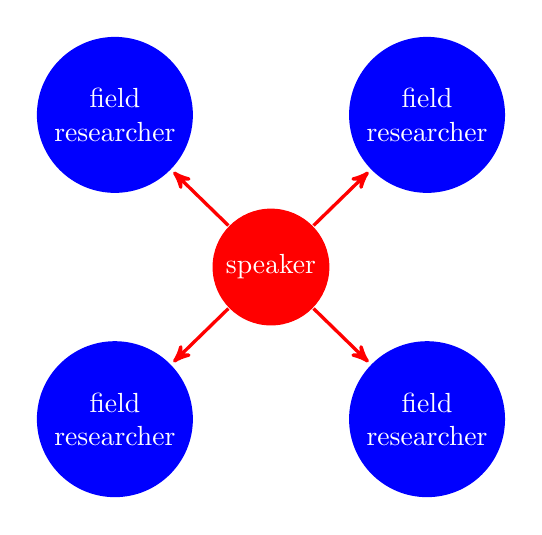
\begin{tikzpicture}[
	  every node/.style={align=center,text=white,draw=none},
	  every matrix/.style={ampersand replacement=\&,column sep=0.25cm,row sep=0.2cm},
	  researcher/.style={thick,circle,fill=blue},
	  speaker/.style={thick,circle,fill=red},
	  revitalizer/.style={thick,regular polygon, regular polygon sides=3,fill=blue,inner sep=-0.2cm},
	  lingsync/.style={thick,fill=green,regular polygon, regular polygon sides=4,inner sep=-.3cm,text=black},
	  documenter/.style={thick,rounded corners,regular polygon, regular polygon sides=4,inner sep=-.2cm,fill=blue},
	  to/.style={->,>=stealth',shorten >=1pt,draw=red,very thick,font=\sffamily\footnotesize}]

	  % Position the nodes using a matrix layout
	  \matrix{
	    \node[researcher] (researchera) {field\\researcher};  \&  \& \node[researcher] (researcherb) {field\\researcher};\\
	      \&  \node[speaker] (speaker) {speaker}; \\
	    \node[researcher] (researcherc) {field\\researcher};  \&  \& \node[researcher] (researcherd) {field\\researcher};\\
	  };
	  \draw[to] (speaker) -- node[midway,right] {} (researchera);
	  \draw[to] (speaker) -- node[midway,left] {} (researcherb);
	  \draw[to] (speaker) -- node[midway,right] {} (researcherc);		  
	  \draw[to] (speaker) -- node[midway,left] {} (researcherd);
\end{tikzpicture}
\end{small}
\end{center}
\end{figure}
\label{fieldwork}
\note{blank note.}
\end{frame}

% GC I added the other steps in the original slides now that we have latex diagrams... not sure if this helps but might be useful for the contextualization in the fieldwork section above instead of some of the text sldies?
\begin{frame}
\frametitle{Collaboration}
\begin{figure}
\begin{center}
\begin{small}
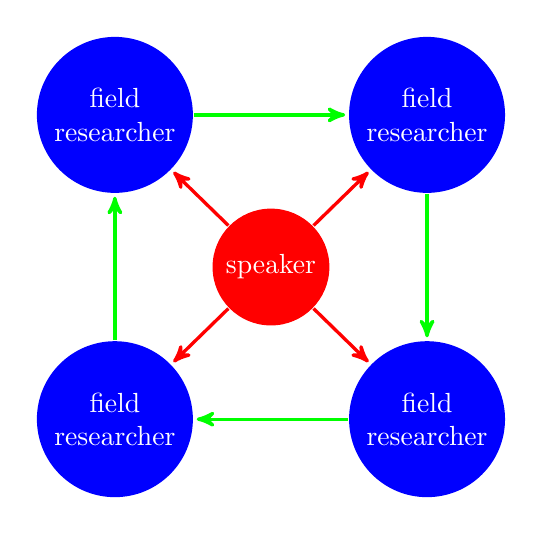
\begin{tikzpicture}[
	  every node/.style={align=center,text=white,draw=none},
	  every matrix/.style={ampersand replacement=\&,column sep=0.25cm,row sep=0.2cm},
	  researcher/.style={thick,circle,fill=blue},
	  speaker/.style={thick,circle,fill=red},
	  revitalizer/.style={thick,regular polygon, regular polygon sides=3,fill=blue,inner sep=-0.2cm},
	  lingsync/.style={thick,fill=green,regular polygon, regular polygon sides=4,inner sep=-.3cm,text=black},
	  documenter/.style={thick,rounded corners,regular polygon, regular polygon sides=4,inner sep=-.2cm,fill=blue},
	  to/.style={->,>=stealth',shorten >=1pt,draw=red,very thick,font=\sffamily\footnotesize},
	  togreen/.style={->,>=stealth',shorten >=1pt,draw=green,very thick,font=\sffamily\footnotesize}]

	  % Position the nodes using a matrix layout
	  \matrix{
	    \node[researcher] (researchera) {field\\researcher};  \&  \& \node[researcher] (researcherb) {field\\researcher};\\
	      \&  \node[speaker] (speaker) {speaker}; \\
	    \node[researcher] (researcherd) {field\\researcher};  \&  \& \node[researcher] (researcherc) {field\\researcher};\\
	  };
	  \draw[to] (speaker) -- node[midway,right] {} (researchera);
	  \draw[to] (speaker) -- node[midway,left] {} (researcherb);
	  \draw[to] (speaker) -- node[midway,right] {} (researcherc);		  
	  \draw[to] (speaker) -- node[midway,left] {} (researcherd);
	  
	  \draw[togreen] (researchera) -- node[midway,left] {} (researcherb);
	  \draw[togreen] (researcherb) -- node[midway,right] {} (researcherc);		  
	  \draw[togreen] (researcherc) -- node[midway,left] {} (researcherd);
	  \draw[togreen] (researcherd) -- node[midway,right] {} (researchera);

\end{tikzpicture}
\end{small}
\end{center}
\end{figure}
\label{fieldworkcollaboration}
\note{blank note.}
\end{frame}


% GC I added the other steps in the original slides now that we have latex diagrams... not sure if this helps but might be useful for the contextualization in the fieldwork section above instead of some of the text sldies?
\begin{frame}
\frametitle{Collaboration}
\begin{figure}
\begin{center}
\begin{small}
\begin{tikzpicture}[
	  every node/.style={align=center,text=white,draw=none},
	  every matrix/.style={ampersand replacement=\&,column sep=0.25cm,row sep=0.2cm},
	  researcher/.style={thick,circle,fill=blue},
%	  fieldwork/.style={thick,regular polygon, regular polygon sides=4,fill=red},
	  fieldwork/.style={thick,fill=red,inner sep=0.3cm},
	  revitalizer/.style={thick,regular polygon, regular polygon sides=3,fill=blue,inner sep=-0.2cm},
	  lingsync/.style={thick,fill=green,regular polygon, regular polygon sides=4,inner sep=-.3cm,text=black},
	  documenter/.style={thick,rounded corners,regular polygon, regular polygon sides=4,inner sep=-.2cm,fill=blue},
	  to/.style={->,>=stealth',shorten >=1pt,draw=red,very thick,font=\sffamily\footnotesize},
	  togreen/.style={->,>=stealth',shorten >=1pt,draw=green,very thick,font=\sffamily\footnotesize}]

	  % Position the nodes using a matrix layout
	  \matrix{
	    \node[researcher] (researchera) {field\\researcher};  \&  \& \node[researcher] (researcherb) {researcher};\\
	      \&  \node[fieldwork] (fieldwork) {fieldwork}; \\
	    \node[documenter] (documenter) {documenter};  \&  \& \node[revitalizer] (revitalizer) {revitalizer};\\
	  };
	  \draw[to] (fieldwork) -- node[midway,right] {} (researchera);
	  \draw[to] (fieldwork) -- node[midway,left] {} (researcherb);
	  \draw[to] (fieldwork) -- node[midway,right] {} (researcherc);		  
	  \draw[to] (fieldwork) -- node[midway,left] {} (researcherd);
	  
	  \draw[togreen] (researchera) -- node[midway,left] {} (researcherb);
	  \draw[togreen] (researcherb) -- node[midway,right] {} (revitalizer);		  
	  \draw[togreen] (revitalizer) -- node[midway,left] {} (documenter);
	  \draw[togreen] (documenter) -- node[midway,right] {} (researchera);

\end{tikzpicture}
\end{small}
\end{center}
\end{figure}
\label{fieldworkexternalcollaboration}
\note{blank note.}
\end{frame}

\begin{frame}
\frametitle{Collaboration}
\begin{figure}
\begin{center}
\begin{small}
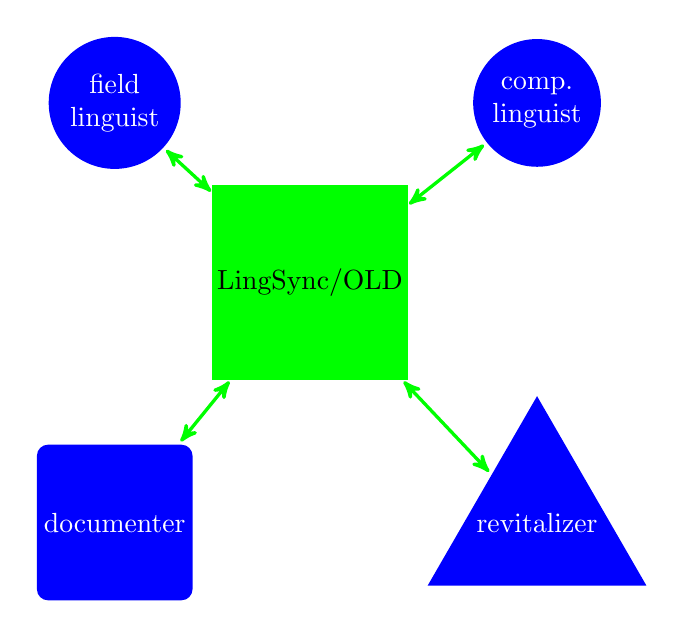
\begin{tikzpicture}[
	  every node/.style={align=center,text=white,draw=none},
	  every matrix/.style={ampersand replacement=\&,column sep=0.25cm,row sep=0.2cm},
	  researcher/.style={thick,circle,fill=blue},
	  revitalizer/.style={thick,regular polygon, regular polygon sides=3,fill=blue,inner sep=-0.2cm},
	  lingsync/.style={thick,fill=green,regular polygon, regular polygon sides=4,inner sep=-.3cm,text=black},
	  documenter/.style={thick,rounded corners,regular polygon, regular polygon sides=4,inner sep=-.2cm,fill=blue},
	  to/.style={<->,>=stealth',shorten >=1pt,draw=green,very thick,font=\sffamily\footnotesize}]

	  % Position the nodes using a matrix layout
	  \matrix{
	    \node[researcher] (researcher1) {field\\linguist};  \&  \& \node[researcher] (researcher2) {comp.\\linguist};\\
	      \&  \node[lingsync] (lingsyncold) {LingSync/OLD}; \\
	    \node[documenter] (documenter) {documenter};  \&  \& \node[revitalizer] (revitalizer) {revitalizer};\\
	  };

	  \draw[to] (lingsyncold) -- node[midway,right] {} (researcher1);
	  \draw[to] (lingsyncold) -- node[midway,left] {} (researcher2);
	  \draw[to] (lingsyncold) -- node[midway,right] {} (documenter);		  
	  \draw[to] (lingsyncold) -- node[midway,left] {} (revitalizer);
\end{tikzpicture}
\end{small}
\label{lingsync:bridge}
\end{center}
\end{figure}
\note[item]{LingSync helps language workers of various types and with
    different goals to share data and collaborate, if they want to.}
\note[item]{As will be discussed on YouTube, the systems offer features and
    conveniences which respond to the requirements of different types
    of fieldworker and fieldwork situation and which may make the system
    worthwhile beyond the primary collaboration- and data-sharing
    functionality.}
\end{frame}



\subsection[Requirements]{Software requirements}


% REQUIREMENTS
%===============================================================================

\begin{frame}

\frametitle{Requirements}
\note[item]<1>{So here we will briefly review the requirements that guided
    the development of LingSync and the OLD.}

\begin{uncoverenv}<2->
\begin{requirement}
\label{req:primary-data}
Integration of primary data
\end{requirement}
\end{uncoverenv}
\note[item]<2>{Rather uncontroversially, the software must be able to handle
    primary data as a first-class citizen of the system. In particular,
    we need to help fieldworkers share audio and video recordings (including
    experimental stimuli). The system should allow for the alignment of
    audio/video with transcriptions and other textual data; the audio/video and
    textual data should be displayed simultaneously for easy cross-reference.
    It should be possible to record audio right into the application and, if
    possible, the text/audio alignment process should be automated or partially
    automated and audio/video should be searchable.}

\begin{uncoverenv}<3->
\begin{requirement}
\label{req:curation}
Curation of data
\end{requirement}
\end{uncoverenv}
\note[item]<3>{The system should facilitate the curation of data, that is, its
    iterative and collaborative refinement over time. For example, the 
    initial output of elicitation could be simply an audio recording, metadata about 
    the source of the recording and a 
    transcription of salient forms. Then, subsequent waves of data curation can
    involve transcription at various levels and/or the creation of
    morphological analyses and annotations of various types, for example,
    tagging and categorizing. Various automations of the data curation process
    are should be easy to script for power users.}


\begin{uncoverenv}<4->
\begin{requirement}
\label{req:inclusive}
Inclusion of stakeholders
\end{requirement}
\end{uncoverenv}
\note[item]<4>{The software should allow for the inclusion of the various
    stakeholders in the endangered languages fieldwork enterprise. That is, the
    software should be useful for language community members, fieldworkers engaged in
    community-based documentation, education, and revitalization projects as well as
    linguistic research teams with members of various types of expertise and
    primary focus (e.g., theoretical, typological, historical, computational)
%    , as well as other
%    disciplines including  translation, language curriculum development which benefit from structured 
%    language data.
     }


\begin{uncoverenv}<5->
\begin{requirement}
\label{req:openable}
Openable data
\end{requirement}
\end{uncoverenv}
\note[item]<5>{The system should allow fieldworkers to produce data which is relatively easy to Open. That
    is, data are available for reuse via various GUIs and APIs while the field work is underway a corpus 
    should also be configurable such that access to portions of the data can be
    restricted to respect licensing and informed consent forms which speakers and communities have requested,
    if necessary.}


\begin{uncoverenv}<6->
\begin{requirement}
\label{req:productivity}
User productivity
\end{requirement}
\end{uncoverenv}
\note[item]<6>{The system should enable user productivity. It should
    include well-designed and cute user interfaces as well as conveniences which speed up 
    repetitive tasks. It should also help with tasks that are particular to
    linguistic fieldwork without making the user interface complex or clunky.}

\end{frame}


\subsection{Existing software}


% EXISTING SOFTWARE
%===============================================================================

\begin{frame}
\frametitle{Existing Software }
\begin{figure}
\begin{center}
\def\firstcircle{(0:-2cm) circle (2.5cm)}
\def\secondcircle{(0:2cm) circle (2.5cm)}
\def\thirdcircle{(0,-2.5cm) circle (2.5cm)} 
\begin{small}
\begin{tikzpicture}
  \draw \firstcircle node {Collaborate};
  \draw \secondcircle node {Features};
  \draw \thirdcircle node {Structure};
  
  \draw (-2cm,0.5cm)  node[text=black] {Share/};
  %\draw (2cm,0.5cm)  node[text=black] {Interlinear Glossing};
  \draw (2cm,0.5cm)  node[text=black] {Fieldwork};

  \draw (4cm,-2cm)  node[text=blue] { \LaTeX};
  \draw (4cm,-3cm)  node[text=blue] {MS Word};

\end{tikzpicture}
\end{small}
\end{center}
\end{figure}
\note[item]{Most field workers use Microsoft Word to type up their data. The user 
  interface is one they already know so there is no training to be done for them to immediately
  begin entering data. While efficient for the needs of field workers the data is difficult to search and reuse by collaborators.}
\end{frame}


\begin{frame}
\frametitle{Existing Software }
\begin{figure}
\begin{center}
\def\firstcircle{(0:-2cm) circle (2.5cm)}
\def\secondcircle{(0:2cm) circle (2.5cm)}
\def\thirdcircle{(0,-2.5cm) circle (2.5cm)} 
\begin{small}
\begin{tikzpicture}
  \draw \firstcircle node {Collaborate};
  \draw \secondcircle node {Features};
  \draw \thirdcircle node {Structure};
  
  \draw (-2cm,0.5cm)  node[text=black] {Share/};
  %\draw (2cm,0.5cm)  node[text=black] {Interlinear Glossing};
  \draw (2cm,0.5cm)  node[text=black] {Fieldwork};


%  \draw (0,-3cm)  node[text=blue] {\tiny Desktop Database Apps};
  \draw (0,-3.5cm)  node[text=blue] {MS Access};
  \draw (0,-4cm)  node[text=blue] {FileMaker Pro};
%  \draw (0,-4cm)  node[text=blue] {\tiny Desktop Spreadsheet };
  \draw (0,-4.5cm)  node[text=blue] {MS Excel};

  \draw (4cm,-2cm)  node[text=blue] { \LaTeX};
  \draw (4cm,-3cm)  node[text=blue] {MS Word};

\end{tikzpicture}
\end{small}
\end{center}
\end{figure}
\note[item]{Microsoft Excel, Microsoft access and FileMaker Pro are more structured and produce data which is easier for computational linguist collaborators to use.}
\end{frame}


\begin{frame}
\frametitle{Existing Software}
\begin{figure}
\begin{center}
\def\firstcircle{(0:-2cm) circle (2.5cm)}
\def\secondcircle{(0:2cm) circle (2.5cm)}
\def\thirdcircle{(0,-2.5cm) circle (2.5cm)} 
\begin{small}
\begin{tikzpicture}
  \draw \firstcircle node {Collaborate};
  \draw \secondcircle node {Features};
  \draw \thirdcircle node {Structure};
  
  \draw (-2cm,0.5cm)  node[text=black] {Share/};
  %\draw (2cm,0.5cm)  node[text=black] {Interlinear Glossing};
  \draw (2cm,0.5cm)  node[text=black] {Fieldwork};
   
  \draw (-2cm,1cm)  node[text=blue] {Google Docs};
  \draw (-1.3cm,-1.3cm)  node[text=blue] {Google};
  \draw (-1.3cm,-1.7cm)  node[text=blue] {Spreadsheets};
  
%  \draw (0,-3cm)  node[text=blue] {\tiny Desktop Database Apps};
  \draw (0,-3.5cm)  node[text=blue] {MS Access};
  \draw (0,-4cm)  node[text=blue] {FileMaker Pro};
%  \draw (0,-4cm)  node[text=blue] {\tiny Desktop Spreadsheet };
  \draw (0,-4.5cm)  node[text=blue] {MS Excel};

  \draw (4cm,-2cm)  node[text=blue] { \LaTeX};
  \draw (4cm,-3cm)  node[text=blue] {MS Word};
\end{tikzpicture}
\end{small}
\end{center}
\end{figure}
\note[item]{Google Docs are better than Microsoft Word in that multiple users can view and edit the data at the same time.}
\note[item]{Google Spreadsheet is even better Google Docs in that the data is structured and can be accessed using a programming interface API.}
\end{frame}


\begin{frame}
\frametitle{Existing Software }
\begin{figure}
\begin{center}
\def\firstcircle{(0:-2cm) circle (2.5cm)}
\def\secondcircle{(0:2cm) circle (2.5cm)}
\def\thirdcircle{(0,-2.5cm) circle (2.5cm)} 
\begin{small}
\begin{tikzpicture}
  \draw \firstcircle node {Collaborate};
  \draw \secondcircle node {Features};
  \draw \thirdcircle node {Structure};
  
  \draw (-2cm,0.5cm)  node[text=black] {Share/};
  %\draw (2cm,0.5cm)  node[text=black] {Interlinear Glossing};
  \draw (2cm,0.5cm)  node[text=black] {Fieldwork};

  \draw (-2cm,1cm)  node[text=blue] {Google Docs};
  \draw (-1.3cm,-1.3cm)  node[text=blue] {Google};
  \draw (-1.3cm,-1.7cm)  node[text=blue] {Spreadsheets};
%  \draw (0,-3cm)  node[text=blue] {\tiny Desktop Database Apps};
  \draw (0,-3.5cm)  node[text=blue] {MS Access};
  \draw (0,-4cm)  node[text=blue] {FileMaker Pro};
%  \draw (0,-4cm)  node[text=blue] {\tiny Desktop Spreadsheet };
  \draw (0,-4.5cm)  node[text=blue] {MS Excel};

  \draw (0.8cm,-1cm)  node[text=blue] {FLEx};
  \draw (1.5cm,-1.5cm)  node[text=blue] {Toolbox};
  \draw (1.2cm,-2cm)  node[text=blue] {ELAN};

  \draw (4cm,-2cm)  node[text=blue] { \LaTeX};
  \draw (4cm,-3cm)  node[text=blue] {MS Word};

\end{tikzpicture}
\end{small}
\label{othersoftware}
\end{center}
\end{figure}
\note[item]{On the other hand we have FLEx, Toolbox, and ELAN which provide features
    specifically designed to facilitate fieldwork tasks: such as 
    presentation of data in IGT format, grammar modelling and automated
    morphological parsing, and export to formats commonly used by linguists.}
\end{frame}


\begin{frame}
\frametitle{Existing Software }
\begin{figure}
\begin{center}
\def\firstcircle{(0:-2cm) circle (2.5cm)}
\def\secondcircle{(0:2cm) circle (2.5cm)}
\def\thirdcircle{(0,-2.5cm) circle (2.5cm)} 
\begin{small}
\begin{tikzpicture}
  \draw \firstcircle node {Collaborate};
  \draw \secondcircle node {Features};
  \draw \thirdcircle node {Structure};
  
  \draw (-2cm,0.5cm)  node[text=black] {Share/};
  %\draw (2cm,0.5cm)  node[text=black] {Interlinear Glossing};
  \draw (2cm,0.5cm)  node[text=black] {Fieldwork};

  \draw (0,-.4cm)  node[text=red] {\tiny LingSync};
  \draw (0,-.6cm)  node[text=red] {\tiny OLD};
  \draw (-2cm,1cm)  node[text=blue] {Google Docs};
  \draw (-1.3cm,-1.3cm)  node[text=blue] {Google};
  \draw (-1.3cm,-1.7cm)  node[text=blue] {Spreadsheets};
%  \draw (0,-3cm)  node[text=blue] {\tiny Desktop Database Apps};
  \draw (0,-3.5cm)  node[text=blue] {MS Access};
  \draw (0,-4cm)  node[text=blue] {FileMaker Pro};
%  \draw (0,-4cm)  node[text=blue] {\tiny Desktop Spreadsheet };
  \draw (0,-4.5cm)  node[text=blue] {MS Excel};

  \draw (0.8cm,-1cm)  node[text=blue] {FLEx};
  \draw (1.5cm,-1.5cm)  node[text=blue] {Toolbox};
  \draw (1.2cm,-2cm)  node[text=blue] {ELAN};

  \draw (4cm,-2cm)  node[text=blue] { \LaTeX};
  \draw (4cm,-3cm)  node[text=blue] {MS Word};

\end{tikzpicture}
\end{small}
\label{othersoftware}
\end{center}
\end{figure}'
\note[item]{Like Google Spreadsheets, LingSync and the OLD allow multiple
     contributors to share data but they also support field work features and integrate well with existing tools for field work.}
\end{frame}


% AD HOC SOLUTIONS --- TODO: I think this frame should maybe be removed
%===============================================================================

\begin{frame}
\frametitle{Ad hoc Solutions}
%TODO will convert into latex diagrams once we are sure we want it.
\begin{figure}
\begin{center}
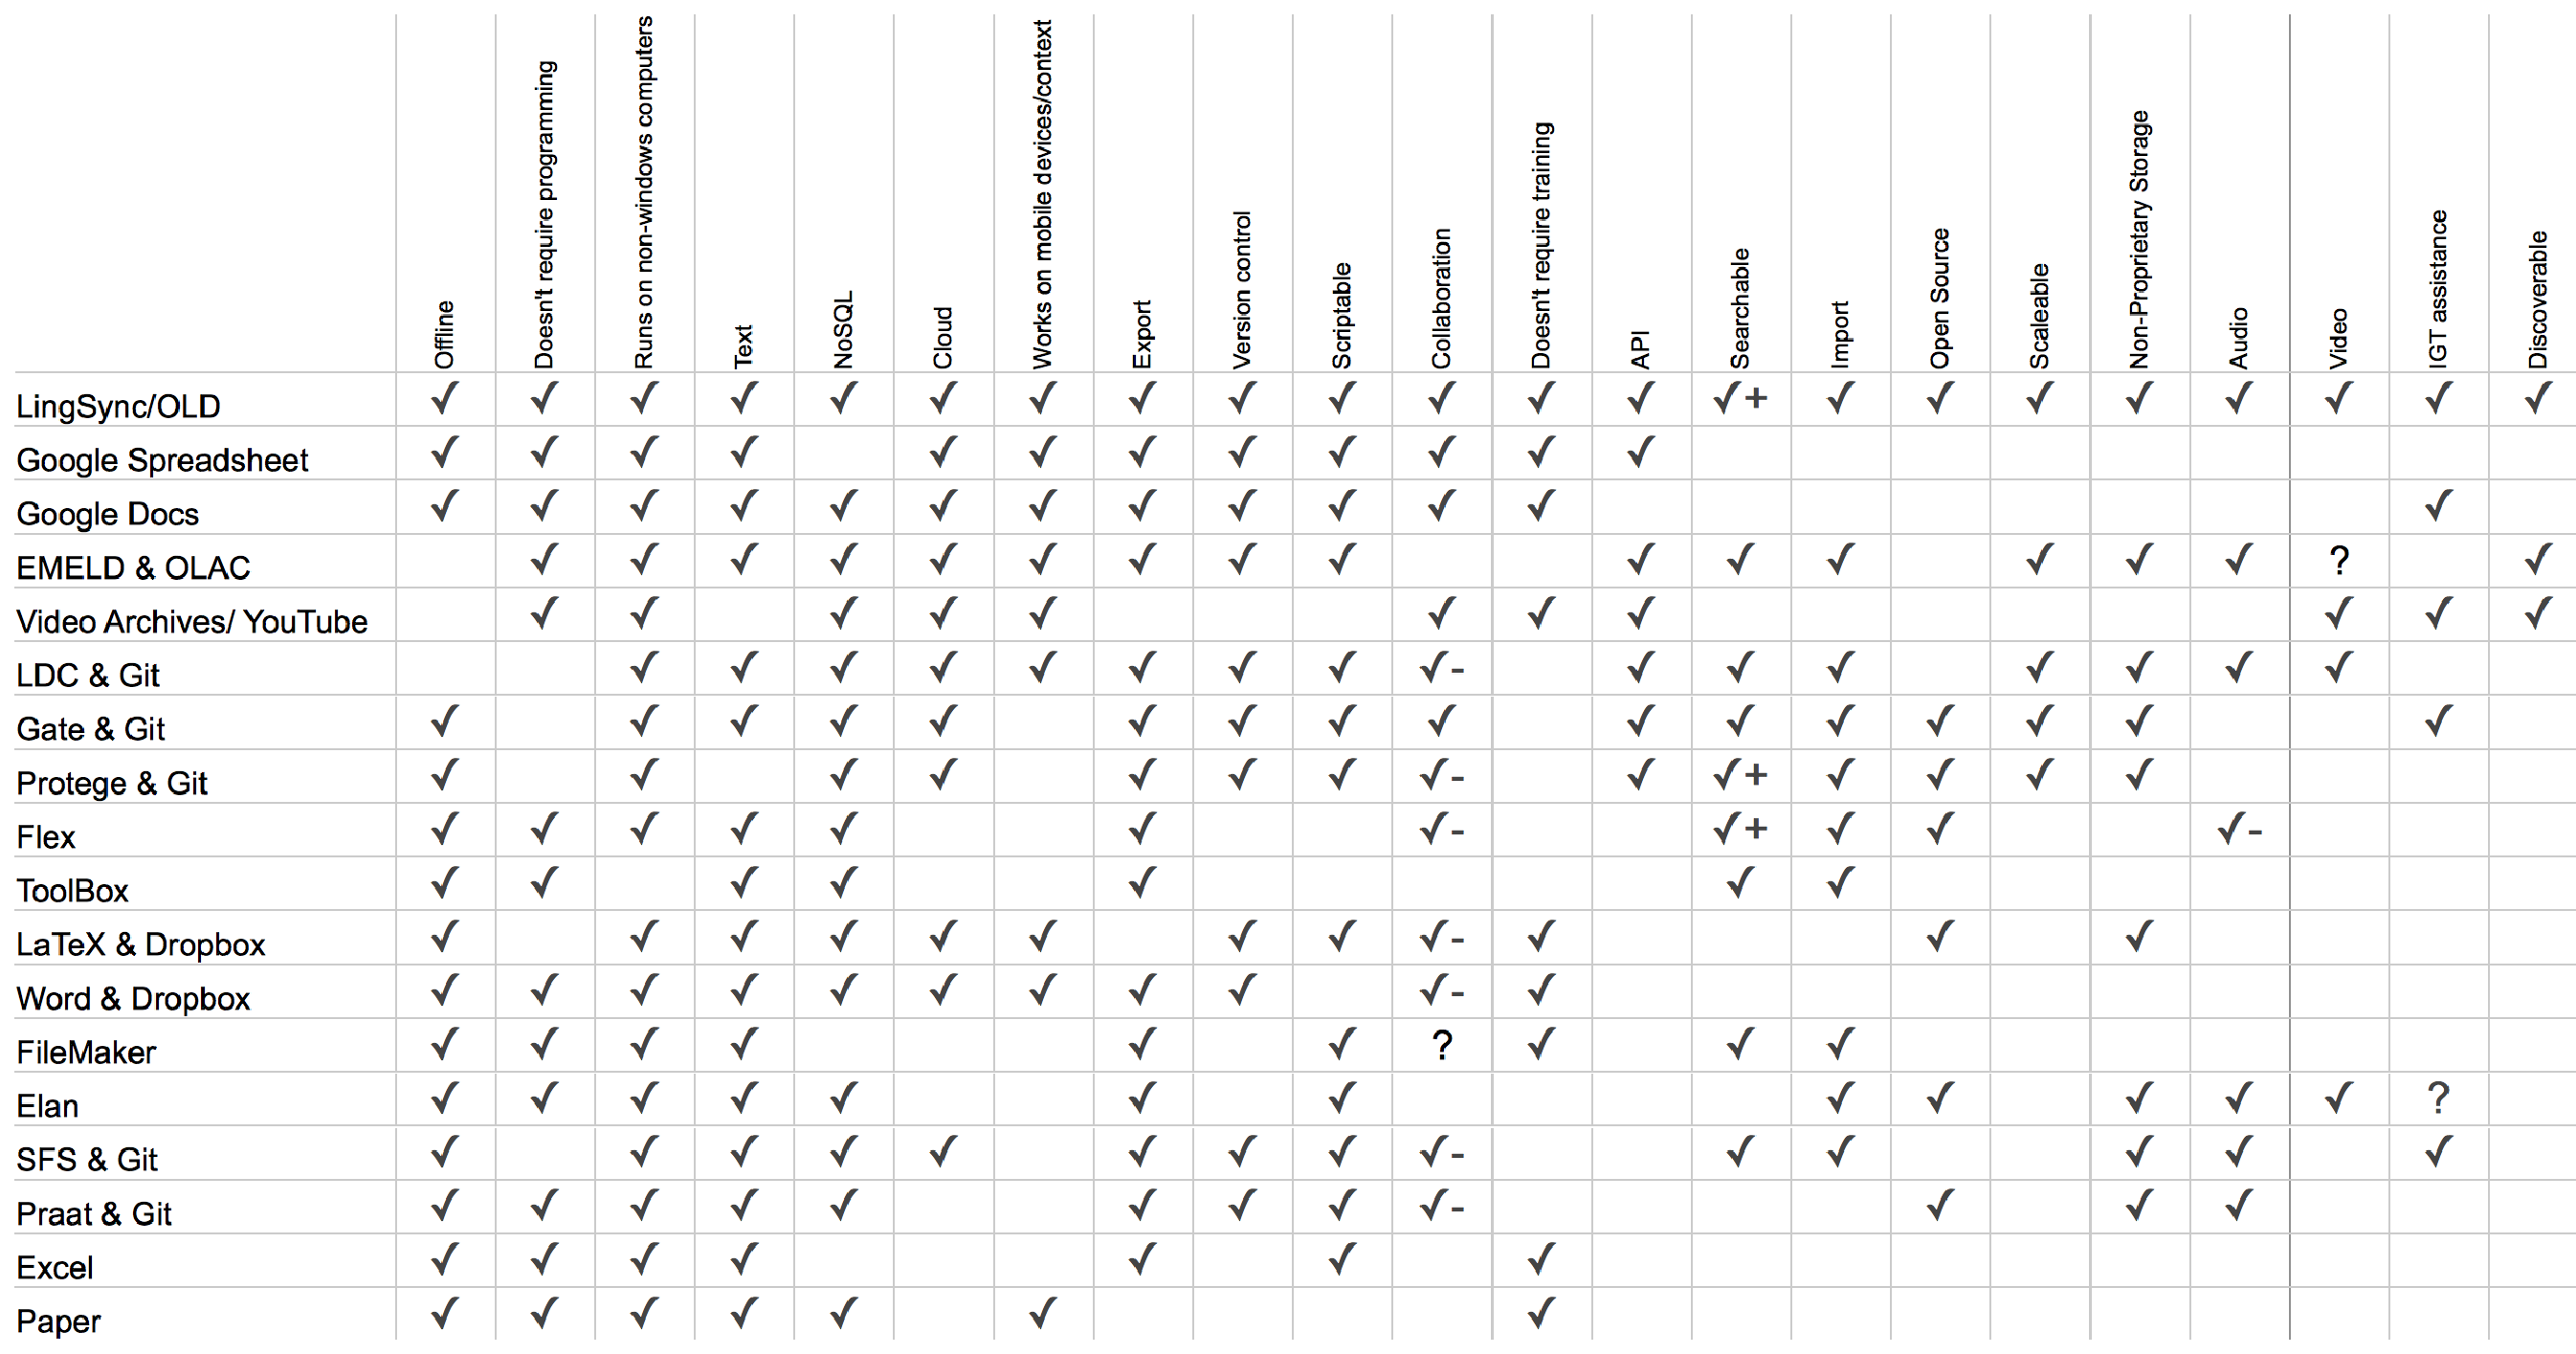
\includegraphics[width=3in]{../figures/other_software}
\caption{Many ad hoc software combinations are used by teams.}
\label{allothersoftware}
\end{center}
\end{figure}
\note[item]{There are more than just three levels of comparison. In this table you can see the multitude of other ad hoc 
    combinations which fieldworkers use to meet their requirements.}
\note[item]{There is no one solution which can facilitate collaborative inclusive curation of data, while fieldwork is underway.}
\note[item]{This is why we began glueing together existing open source modules and providing cute user interfaces to create what has come to be LingSync.}
\end{frame}


\section[LingSync/OLD]{New models for data collection and management}
\subsection{Architecture}\label{sec:lingsync}

% LATEX GRAPHIC COMMENTED OUT BECAUSE I DON'T UNDERSTAND THE "PHONETIC" BOX

% GC I added some more frames from the why lingsync slides, you can comment them out if you want
\begin{frame}
\frametitle{LingSync Architecture}
\begin{figure}
\begin{center}
\begin{small}
\tikzstyle{todouble} = [thick, green,decoration={markings,mark=at position
   1 with {\arrow[thick,green]{ triangle 60}}},
   double distance=4pt, shorten >= 8pt,
   preaction = {decorate},
   postaction = {draw,line width=4pt, green, shorten >= 8pt}]

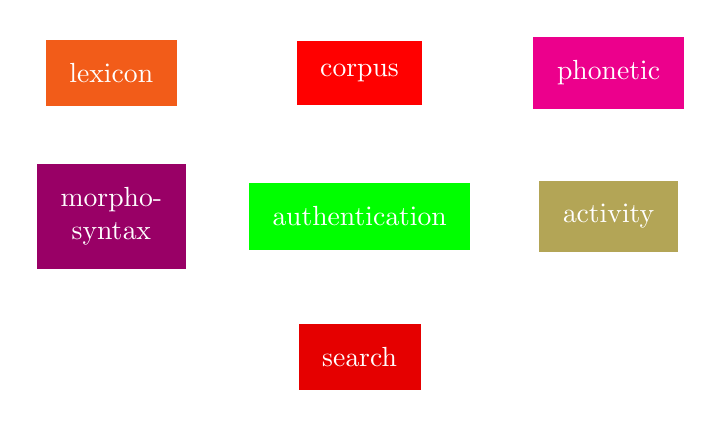
\begin{tikzpicture}[
	  every node/.style={align=center,text=white,draw=none},
	  every matrix/.style={ampersand replacement=\&,column sep=0.8cm,row sep=0.7cm},
	  audio/.style={thick,fill=magenta,inner sep=0.3cm},
	  corpus/.style={thick,fill=red,inner sep=0.3cm},
	  lexicon/.style={thick,fill=yellow!30!red,inner sep=0.3cm},
	  parser/.style={thick,fill=blue!40!red,inner sep=0.3cm},
	  authentication/.style={thick,fill=green,inner sep=0.3cm},
	  activity/.style={thick,fill=yellow!70!blue,inner sep=0.3cm},
	  search/.style={thick,fill=black!10!red,inner sep=0.3cm},
	  revitalizer/.style={thick,regular polygon, regular polygon sides=3,fill=black!60!green, inner sep=0cm},
	  researcher/.style={thick,circle,fill=black},
	  documenter/.style={thick,rounded corners,regular polygon, regular polygon sides=4,fill=blue, inner sep=0cm},
	  to/.style={->,>=stealth',shorten >=1pt,draw=green,very thick,font=\sffamily\footnotesize},
	  twoway/.style={<->,>=stealth',shorten >=1pt,draw=green,very thick,font=\sffamily\footnotesize}]

	  % Position the nodes using a matrix layout
	  \matrix{
	     \node[lexicon] (lexicon) {lexicon};  \&   \node[corpus] (corpus) {corpus};  \& \node[audio] (audio) {phonetic};   \\
	    	    \node[parser] (parser) {morpho-\\syntax}; \&  \node[authentication] (authentication) {authentication}; \& \node[activity] (activity) {activity};\\
		    \& \node[search] (search) {search};\\
	    };
\end{tikzpicture}
\end{small}
\label{lingsync:webservices}
\end{center}
\end{figure}
\note{LingSync has many web services}
\end{frame}


% GC I added some more frames from the why lingsync slides, you can comment them out if you want
\begin{frame}
\frametitle{LingSync Architecture}
\begin{figure}
\begin{center}
\begin{small}
\tikzstyle{todouble} = [thick, green,decoration={markings,mark=at position
   1 with {\arrow[thick,green]{ triangle 60}}},
   double distance=4pt, shorten >= 8pt,
   preaction = {decorate},
   postaction = {draw,line width=4pt, green, shorten >= 8pt}]

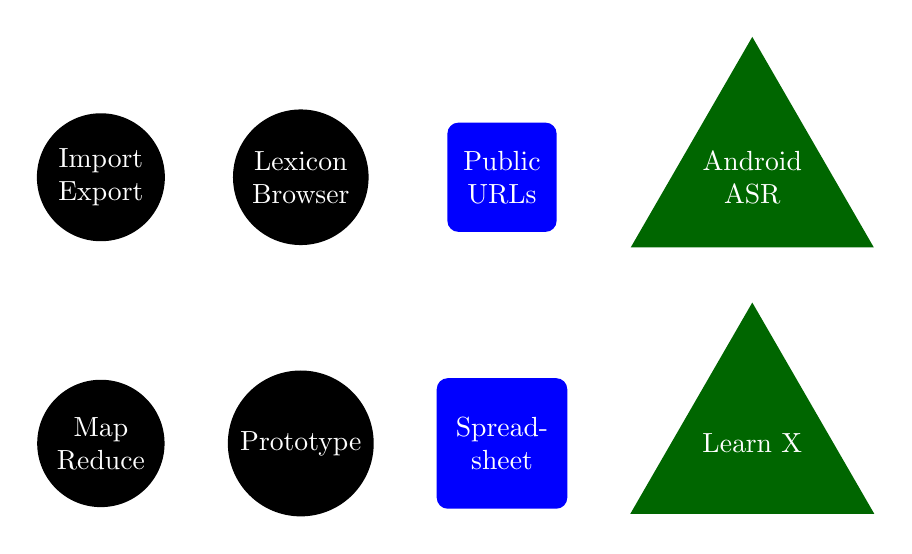
\begin{tikzpicture}[
	  every node/.style={align=center,text=white,draw=none},
	  every matrix/.style={ampersand replacement=\&,column sep=0.8cm,row sep=0.7cm},
	  audio/.style={thick,fill=magenta,inner sep=0.3cm},
	  corpus/.style={thick,fill=red,inner sep=0.3cm},
	  lexicon/.style={thick,fill=yellow!30!red,inner sep=0.3cm},
	  parser/.style={thick,fill=blue!40!red,inner sep=0.3cm},
	  activity/.style={thick,fill=green,inner sep=0.3cm},
	  revitalizer/.style={thick,regular polygon, regular polygon sides=3,fill=black!60!green, inner sep=0cm},
	  researcher/.style={thick,circle,fill=black},
	  documenter/.style={thick,rounded corners,regular polygon, regular polygon sides=4,fill=blue, inner sep=0cm},
	  to/.style={->,>=stealth',shorten >=1pt,draw=green,very thick,font=\sffamily\footnotesize},
	  twoway/.style={<->,>=stealth',shorten >=1pt,draw=green,very thick,font=\sffamily\footnotesize}]

	  % Position the nodes using a matrix layout
	  \matrix{
	  \node[researcher] (importexport) {Import\\Export}; \& \node[researcher] (lexbrowser) {Lexicon\\Browser};  \& \node[documenter] (corpuspages) {Public\\URLs}; \& \node[revitalizer] (asr) {Android\\ASR};\\
	   \node[researcher] (mapreduce) {Map\\Reduce}; \& \node[researcher] (prototype) {Prototype};  \& \node[documenter] (spreadsheet) {Spread-\\sheet};  \& \node[revitalizer] (learnx) {Learn X};  \\
	  };

\end{tikzpicture}
\end{small}
\label{lingsync:uis}
\end{center}
\end{figure}
\note{And many user interfaces for different stakeholders, in both mobile and desktop contexts}
\end{frame}

% GC I added some more frames from the why lingsync slides, you can comment them out if you want
\begin{frame}
\frametitle{LingSync Architecture}
\begin{figure}
\begin{center}
\begin{small}
\tikzstyle{todouble} = [thick, green,decoration={markings,mark=at position
   1 with {\arrow[thick,green]{ triangle 60}}},
   double distance=4pt, shorten >= 8pt,
   preaction = {decorate},
   postaction = {draw,line width=4pt, green, shorten >= 8pt}]

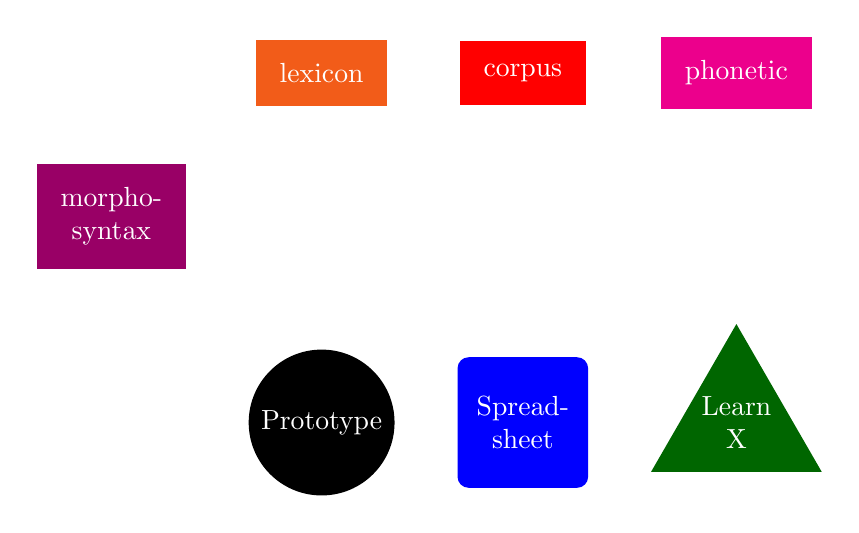
\begin{tikzpicture}[
	  every node/.style={align=center,text=white,draw=none},
	  every matrix/.style={ampersand replacement=\&,column sep=0.8cm,row sep=0.7cm},
	  audio/.style={thick,fill=magenta,inner sep=0.3cm},
	  corpus/.style={thick,fill=red,inner sep=0.3cm},
	  lexicon/.style={thick,fill=yellow!30!red,inner sep=0.3cm},
	  parser/.style={thick,fill=blue!40!red,inner sep=0.3cm},
	  activity/.style={thick,fill=green,inner sep=0.3cm},
	  revitalizer/.style={thick,regular polygon, regular polygon sides=3,fill=black!60!green, inner sep=0cm},
	  researcher/.style={thick,circle,fill=black},
	  documenter/.style={thick,rounded corners,regular polygon, regular polygon sides=4,fill=blue, inner sep=0cm},
	  to/.style={->,>=stealth',shorten >=1pt,draw=green,very thick,font=\sffamily\footnotesize},
	  twoway/.style={<->,>=stealth',shorten >=1pt,draw=green,very thick,font=\sffamily\footnotesize}]

	  % Position the nodes using a matrix layout
	  \matrix{
	    \&  \node[lexicon] (lexicon) {lexicon};  \&   \node[corpus] (corpus) {corpus};  \& \node[audio] (audio) {phonetic};   \\
	    \node[parser] (parser) {morpho-\\syntax}; \& \& \&\\ %\node[activity] (activity) {activity};\\
	    \&  \node[researcher] (prototype) {Prototype};  \& \node[documenter] (spreadsheet) {Spread-\\sheet};  \& \node[revitalizer] (learnx) {Learn\\X};  \\
	  };

\end{tikzpicture}
\end{small}
\label{lingsync:architecture}
\end{center}
\end{figure}
\note{Lets look how the core web services and user interfaces}
\end{frame}

% GC I added some more frames from the why lingsync slides, you can comment them out if you want
\begin{frame}
\frametitle{LingSync Architecture}
\begin{figure}
\begin{center}
\begin{small}
\tikzstyle{todouble} = [thick, green,decoration={markings,mark=at position
   1 with {\arrow[thick,green]{ triangle 60}}},
   double distance=4pt, shorten >= 8pt,
   preaction = {decorate},
   postaction = {draw,line width=4pt, green, shorten >= 8pt}]

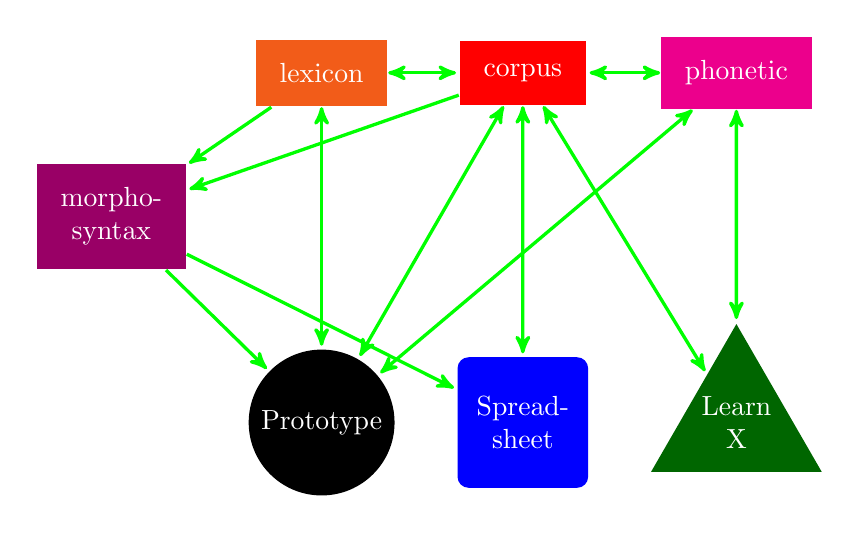
\begin{tikzpicture}[
	  every node/.style={align=center,text=white,draw=none},
	  every matrix/.style={ampersand replacement=\&,column sep=0.8cm,row sep=0.7cm},
	  audio/.style={thick,fill=magenta,inner sep=0.3cm},
	  corpus/.style={thick,fill=red,inner sep=0.3cm},
	  lexicon/.style={thick,fill=yellow!30!red,inner sep=0.3cm},
	  parser/.style={thick,fill=blue!40!red,inner sep=0.3cm},
	  activity/.style={thick,fill=green,inner sep=0.3cm},
	  revitalizer/.style={thick,regular polygon, regular polygon sides=3,fill=black!60!green, inner sep=0cm},
	  researcher/.style={thick,circle,fill=black},
	  documenter/.style={thick,rounded corners,regular polygon, regular polygon sides=4,fill=blue, inner sep=0cm},
	  to/.style={->,>=stealth',shorten >=1pt,draw=green,very thick,font=\sffamily\footnotesize},
	  twoway/.style={<->,>=stealth',shorten >=1pt,draw=green,very thick,font=\sffamily\footnotesize}]

	  % Position the nodes using a matrix layout
	  \matrix{
	    \&  \node[lexicon] (lexicon) {lexicon};  \&   \node[corpus] (corpus) {corpus};  \& \node[audio] (audio) {phonetic};   \\
	    \node[parser] (parser) {morpho-\\syntax}; \& \& \&\\ %\node[activity] (activity) {activity};\\
	    \&  \node[researcher] (prototype) {Prototype};  \& \node[documenter] (spreadsheet) {Spread-\\sheet};  \& \node[revitalizer] (learnx) {Learn\\X};  \\
% Actually there are more UIs:
%	   \node[researcher] (lexbrowser) {Lexicon\\Browser};   \&  \node[researcher] (prototype) {Prototype};  \& \node[documenter] (spreadsheet) {Spread-\\sheet};  \& \node[documenter] (corpuspages) {Public\\URLs};  \& \node[revitalizer] (learnx) {learnx};  \& \node[revitalizer] (asr) {ASR};\\
	  };

	  \draw[twoway] (lexicon) -- node[midway,right] {} (corpus);
	  \draw[twoway] (audio) -- node[midway,right] {} (corpus);
	  \draw[to] (lexicon) -- node[midway] {} (parser);
	  \draw[to] (corpus) -- node[midway] {} (parser);
	  \draw[to] (parser) -- node[midway,right] {} (prototype);
	  \draw[to] (parser) -- node[midway,right] {} (spreadsheet);
	  \draw[twoway] (corpus) -- node[midway,right] {} (prototype);
	  \draw[twoway] (corpus) -- node[midway,right] {} (spreadsheet);
	  \draw[twoway] (corpus) -- node[midway,right] {} (learnx);
	  \draw[twoway] (audio) -- node[midway,right] {} (prototype);
%	  \draw[twoway] (audio) -- node[midway,right] {} (spreadsheet); %TODO its not supposed to be missing this arrow, it just happened as the app was being developed... the spreadsheet DOES have audio, but the audio is going straight into the corpus rather than being preprocessed.
	  \draw[twoway] (audio) -- node[midway,right] {} (learnx);
	  \draw[twoway] (lexicon) -- node[midway,right] {} (prototype);
\end{tikzpicture}
\end{small}
\label{lingsync:architecture}
\end{center}
\end{figure}
\note{ are connected}
\end{frame}

% GC I added some more frames from the why lingsync slides, you can comment them out if you want
\begin{frame}
\frametitle{LingSync Architecture}
\begin{figure}
\begin{center}
\begin{tabular}{lll}
* many platforms \\
\end{tabular}
\begin{small}
\tikzstyle{todouble} = [thick, green,decoration={markings,mark=at position
   1 with {\arrow[thick,green]{ triangle 60}}},
   double distance=4pt, shorten >= 8pt,
   preaction = {decorate},
   postaction = {draw,line width=4pt, green, shorten >= 8pt}]

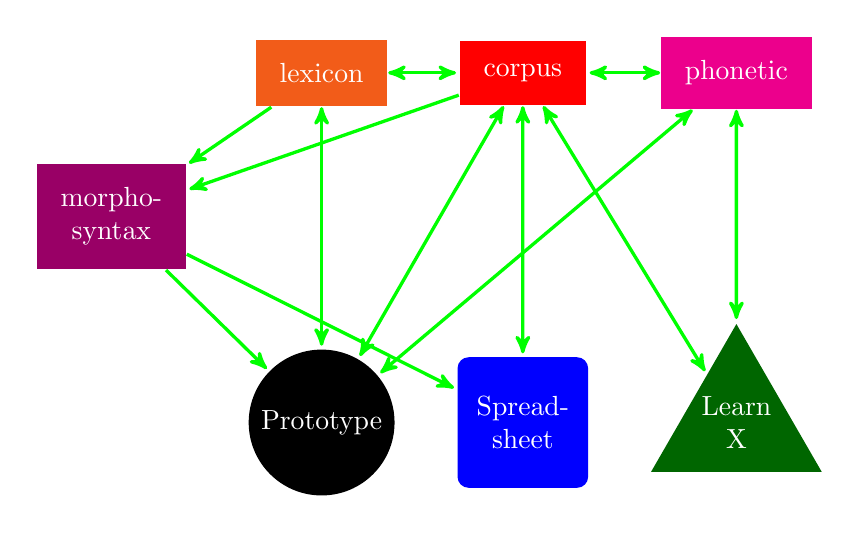
\begin{tikzpicture}[
	  every node/.style={align=center,text=white,draw=none},
	  every matrix/.style={ampersand replacement=\&,column sep=0.8cm,row sep=0.7cm},
	  audio/.style={thick,fill=magenta,inner sep=0.3cm},
	  corpus/.style={thick,fill=red,inner sep=0.3cm},
	  lexicon/.style={thick,fill=yellow!30!red,inner sep=0.3cm},
	  parser/.style={thick,fill=blue!40!red,inner sep=0.3cm},
	  activity/.style={thick,fill=green,inner sep=0.3cm},
	  revitalizer/.style={thick,regular polygon, regular polygon sides=3,fill=black!60!green, inner sep=0cm},
	  researcher/.style={thick,circle,fill=black},
	  documenter/.style={thick,rounded corners,regular polygon, regular polygon sides=4,fill=blue, inner sep=0cm},
	  to/.style={->,>=stealth',shorten >=1pt,draw=green,very thick,font=\sffamily\footnotesize},
	  twoway/.style={<->,>=stealth',shorten >=1pt,draw=green,very thick,font=\sffamily\footnotesize}]

	  % Position the nodes using a matrix layout
	  \matrix{
	    \&  \node[lexicon] (lexicon) {lexicon};  \&   \node[corpus] (corpus) {corpus};  \& \node[audio] (audio) {phonetic};   \\
	    \node[parser] (parser) {morpho-\\syntax}; \& \& \&\\ %\node[activity] (activity) {activity};\\
	    \&  \node[researcher] (prototype) {Prototype};  \& \node[documenter] (spreadsheet) {Spread-\\sheet};  \& \node[revitalizer] (learnx) {Learn\\X};  \\
% Actually there are more UIs:
%	   \node[researcher] (lexbrowser) {Lexicon\\Browser};   \&  \node[researcher] (prototype) {Prototype};  \& \node[documenter] (spreadsheet) {Spread-\\sheet};  \& \node[documenter] (corpuspages) {Public\\URLs};  \& \node[revitalizer] (learnx) {learnx};  \& \node[revitalizer] (asr) {ASR};\\
	  };

	  \draw[twoway] (lexicon) -- node[midway,right] {} (corpus);
	  \draw[twoway] (audio) -- node[midway,right] {} (corpus);
	  \draw[to] (lexicon) -- node[midway] {} (parser);
	  \draw[to] (corpus) -- node[midway] {} (parser);
	  \draw[to] (parser) -- node[midway,right] {} (prototype);
	  \draw[to] (parser) -- node[midway,right] {} (spreadsheet);
	  \draw[twoway] (corpus) -- node[midway,right] {} (prototype);
	  \draw[twoway] (corpus) -- node[midway,right] {} (spreadsheet);
	  \draw[twoway] (corpus) -- node[midway,right] {} (learnx);
	  \draw[twoway] (audio) -- node[midway,right] {} (prototype);
%	  \draw[twoway] (audio) -- node[midway,right] {} (spreadsheet); %TODO its not supposed to be missing this arrow, it just happened as the app was being developed... the spreadsheet DOES have audio, but the audio is going straight into the corpus rather than being preprocessed.
	  \draw[twoway] (audio) -- node[midway,right] {} (learnx);
	  \draw[twoway] (lexicon) -- node[midway,right] {} (prototype);
\end{tikzpicture}
\end{small}
\label{lingsync:architecture}
\end{center}
\end{figure}
\note{to serve many platforms}
\end{frame}

% GC I added some more frames from the why lingsync slides, you can comment them out if you want
\begin{frame}
\frametitle{LingSync Architecture}
\begin{figure}
\begin{center}
\begin{tabular}{lll}
* many platforms  & * online/offline \\
\end{tabular}
\begin{small}
\tikzstyle{todouble} = [thick, green,decoration={markings,mark=at position
   1 with {\arrow[thick,green]{ triangle 60}}},
   double distance=4pt, shorten >= 8pt,
   preaction = {decorate},
   postaction = {draw,line width=4pt, green, shorten >= 8pt}]

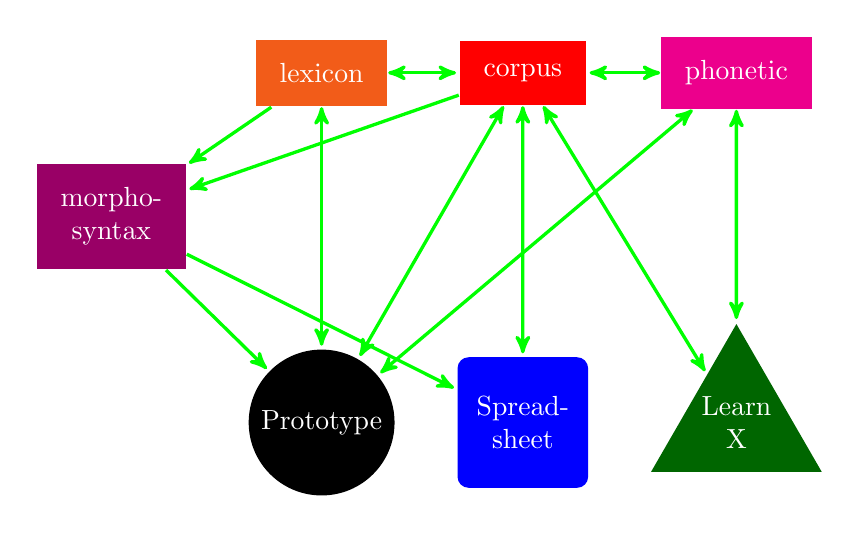
\begin{tikzpicture}[
	  every node/.style={align=center,text=white,draw=none},
	  every matrix/.style={ampersand replacement=\&,column sep=0.8cm,row sep=0.7cm},
	  audio/.style={thick,fill=magenta,inner sep=0.3cm},
	  corpus/.style={thick,fill=red,inner sep=0.3cm},
	  lexicon/.style={thick,fill=yellow!30!red,inner sep=0.3cm},
	  parser/.style={thick,fill=blue!40!red,inner sep=0.3cm},
	  activity/.style={thick,fill=green,inner sep=0.3cm},
	  revitalizer/.style={thick,regular polygon, regular polygon sides=3,fill=black!60!green, inner sep=0cm},
	  researcher/.style={thick,circle,fill=black},
	  documenter/.style={thick,rounded corners,regular polygon, regular polygon sides=4,fill=blue, inner sep=0cm},
	  to/.style={->,>=stealth',shorten >=1pt,draw=green,very thick,font=\sffamily\footnotesize},
	  twoway/.style={<->,>=stealth',shorten >=1pt,draw=green,very thick,font=\sffamily\footnotesize}]

	  % Position the nodes using a matrix layout
	  \matrix{
	    \&  \node[lexicon] (lexicon) {lexicon};  \&   \node[corpus] (corpus) {corpus};  \& \node[audio] (audio) {phonetic};   \\
	    \node[parser] (parser) {morpho-\\syntax}; \& \& \&\\ %\node[activity] (activity) {activity};\\
	    \&  \node[researcher] (prototype) {Prototype};  \& \node[documenter] (spreadsheet) {Spread-\\sheet};  \& \node[revitalizer] (learnx) {Learn\\X};  \\
% Actually there are more UIs:
%	   \node[researcher] (lexbrowser) {Lexicon\\Browser};   \&  \node[researcher] (prototype) {Prototype};  \& \node[documenter] (spreadsheet) {Spread-\\sheet};  \& \node[documenter] (corpuspages) {Public\\URLs};  \& \node[revitalizer] (learnx) {learnx};  \& \node[revitalizer] (asr) {ASR};\\
	  };

	  \draw[twoway] (lexicon) -- node[midway,right] {} (corpus);
	  \draw[twoway] (audio) -- node[midway,right] {} (corpus);
	  \draw[to] (lexicon) -- node[midway] {} (parser);
	  \draw[to] (corpus) -- node[midway] {} (parser);
	  \draw[to] (parser) -- node[midway,right] {} (prototype);
	  \draw[to] (parser) -- node[midway,right] {} (spreadsheet);
	  \draw[twoway] (corpus) -- node[midway,right] {} (prototype);
	  \draw[twoway] (corpus) -- node[midway,right] {} (spreadsheet);
	  \draw[twoway] (corpus) -- node[midway,right] {} (learnx);
	  \draw[twoway] (audio) -- node[midway,right] {} (prototype);
%	  \draw[twoway] (audio) -- node[midway,right] {} (spreadsheet); %TODO its not supposed to be missing this arrow, it just happened as the app was being developed... the spreadsheet DOES have audio, but the audio is going straight into the corpus rather than being preprocessed.
	  \draw[twoway] (audio) -- node[midway,right] {} (learnx);
	  \draw[twoway] (lexicon) -- node[midway,right] {} (prototype);
\end{tikzpicture}
\end{small}
\label{lingsync:architecture}
\end{center}
\end{figure}
\note{in online, offline and low bandwidth situations}
\end{frame}



% GC I added some more frames from the why lingsync slides, you can comment them out if you want
\begin{frame}
\frametitle{LingSync Architecture}
\begin{figure}
\begin{center}
\begin{tabular}{lll}
* many platforms  & * online/offline \\
* many purposes
\end{tabular}
\begin{small}
\tikzstyle{todouble} = [thick, green,decoration={markings,mark=at position
   1 with {\arrow[thick,green]{ triangle 60}}},
   double distance=4pt, shorten >= 8pt,
   preaction = {decorate},
   postaction = {draw,line width=4pt, green, shorten >= 8pt}]

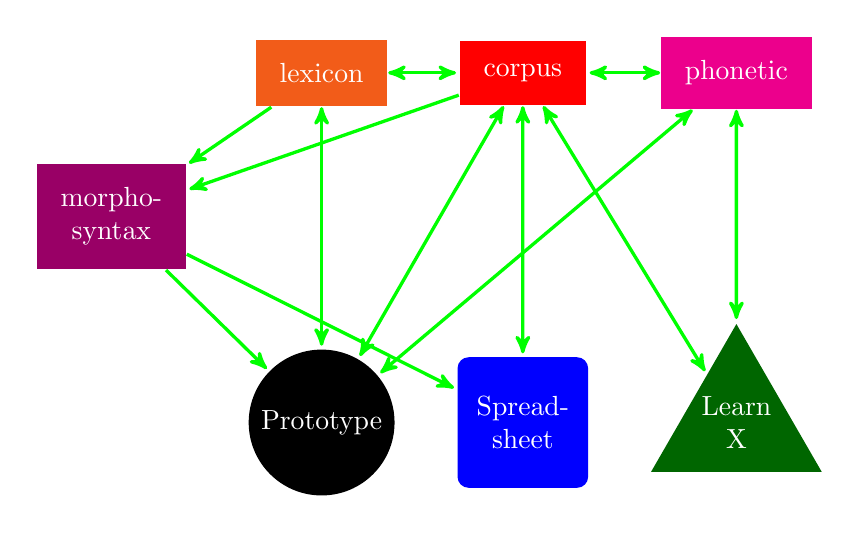
\begin{tikzpicture}[
	  every node/.style={align=center,text=white,draw=none},
	  every matrix/.style={ampersand replacement=\&,column sep=0.8cm,row sep=0.7cm},
	  audio/.style={thick,fill=magenta,inner sep=0.3cm},
	  corpus/.style={thick,fill=red,inner sep=0.3cm},
	  lexicon/.style={thick,fill=yellow!30!red,inner sep=0.3cm},
	  parser/.style={thick,fill=blue!40!red,inner sep=0.3cm},
	  activity/.style={thick,fill=green,inner sep=0.3cm},
	  revitalizer/.style={thick,regular polygon, regular polygon sides=3,fill=black!60!green, inner sep=0cm},
	  researcher/.style={thick,circle,fill=black},
	  documenter/.style={thick,rounded corners,regular polygon, regular polygon sides=4,fill=blue, inner sep=0cm},
	  to/.style={->,>=stealth',shorten >=1pt,draw=green,very thick,font=\sffamily\footnotesize},
	  twoway/.style={<->,>=stealth',shorten >=1pt,draw=green,very thick,font=\sffamily\footnotesize}]

	  % Position the nodes using a matrix layout
	  \matrix{
	    \&  \node[lexicon] (lexicon) {lexicon};  \&   \node[corpus] (corpus) {corpus};  \& \node[audio] (audio) {phonetic};   \\
	    \node[parser] (parser) {morpho-\\syntax}; \& \& \&\\ %\node[activity] (activity) {activity};\\
	    \&  \node[researcher] (prototype) {Prototype};  \& \node[documenter] (spreadsheet) {Spread-\\sheet};  \& \node[revitalizer] (learnx) {Learn\\X};  \\
% Actually there are more UIs:
%	   \node[researcher] (lexbrowser) {Lexicon\\Browser};   \&  \node[researcher] (prototype) {Prototype};  \& \node[documenter] (spreadsheet) {Spread-\\sheet};  \& \node[documenter] (corpuspages) {Public\\URLs};  \& \node[revitalizer] (learnx) {learnx};  \& \node[revitalizer] (asr) {ASR};\\
	  };

	  \draw[twoway] (lexicon) -- node[midway,right] {} (corpus);
	  \draw[twoway] (audio) -- node[midway,right] {} (corpus);
	  \draw[to] (lexicon) -- node[midway] {} (parser);
	  \draw[to] (corpus) -- node[midway] {} (parser);
	  \draw[to] (parser) -- node[midway,right] {} (prototype);
	  \draw[to] (parser) -- node[midway,right] {} (spreadsheet);
	  \draw[twoway] (corpus) -- node[midway,right] {} (prototype);
	  \draw[twoway] (corpus) -- node[midway,right] {} (spreadsheet);
	  \draw[twoway] (corpus) -- node[midway,right] {} (learnx);
	  \draw[twoway] (audio) -- node[midway,right] {} (prototype);
%	  \draw[twoway] (audio) -- node[midway,right] {} (spreadsheet); %TODO its not supposed to be missing this arrow, it just happened as the app was being developed... the spreadsheet DOES have audio, but the audio is going straight into the corpus rather than being preprocessed.
	  \draw[twoway] (audio) -- node[midway,right] {} (learnx);
	  \draw[twoway] (lexicon) -- node[midway,right] {} (prototype);
\end{tikzpicture}
\end{small}
\label{lingsync:architecture}
\end{center}
\end{figure}
\note{letting the data grow for teams with many purposes}
\end{frame}


% GC I added some more frames from the why lingsync slides, you can comment them out if you want
\begin{frame}
\frametitle{LingSync Architecture}
\begin{figure}
\begin{center}
\begin{tabular}{lll}
* many platforms & * online/offline\\
* many purposes & * extendable
\end{tabular}
\begin{small}
\tikzstyle{todouble} = [thick, green,decoration={markings,mark=at position
   1 with {\arrow[thick,green]{ triangle 60}}},
   double distance=4pt, shorten >= 8pt,
   preaction = {decorate},
   postaction = {draw,line width=4pt, green, shorten >= 8pt}]

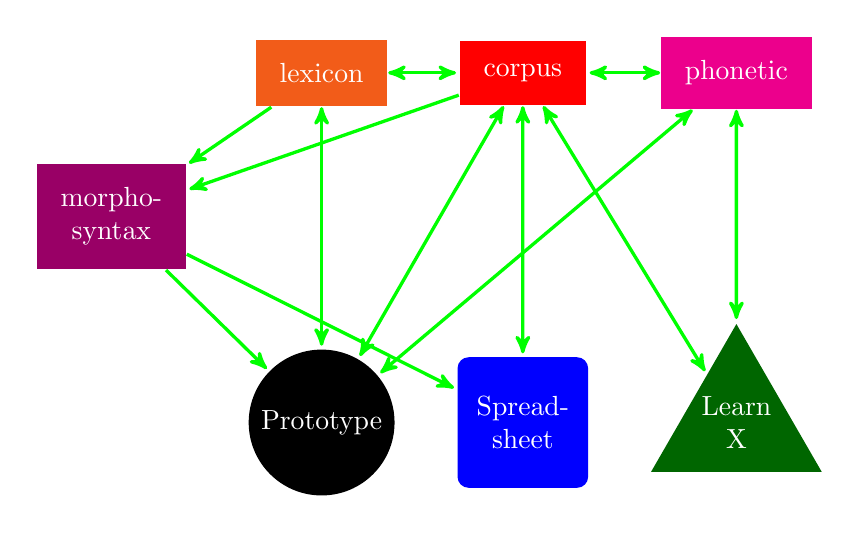
\begin{tikzpicture}[
	  every node/.style={align=center,text=white,draw=none},
	  every matrix/.style={ampersand replacement=\&,column sep=0.8cm,row sep=0.7cm},
	  audio/.style={thick,fill=magenta,inner sep=0.3cm},
	  corpus/.style={thick,fill=red,inner sep=0.3cm},
	  lexicon/.style={thick,fill=yellow!30!red,inner sep=0.3cm},
	  parser/.style={thick,fill=blue!40!red,inner sep=0.3cm},
	  activity/.style={thick,fill=green,inner sep=0.3cm},
	  revitalizer/.style={thick,regular polygon, regular polygon sides=3,fill=black!60!green, inner sep=0cm},
	  researcher/.style={thick,circle,fill=black},
	  documenter/.style={thick,rounded corners,regular polygon, regular polygon sides=4,fill=blue, inner sep=0cm},
	  to/.style={->,>=stealth',shorten >=1pt,draw=green,very thick,font=\sffamily\footnotesize},
	  twoway/.style={<->,>=stealth',shorten >=1pt,draw=green,very thick,font=\sffamily\footnotesize}]

	  % Position the nodes using a matrix layout
	  \matrix{
	    \&  \node[lexicon] (lexicon) {lexicon};  \&   \node[corpus] (corpus) {corpus};  \& \node[audio] (audio) {phonetic};   \\
	    \node[parser] (parser) {morpho-\\syntax}; \& \& \&\\ %\node[activity] (activity) {activity};\\
	    \&  \node[researcher] (prototype) {Prototype};  \& \node[documenter] (spreadsheet) {Spread-\\sheet};  \& \node[revitalizer] (learnx) {Learn\\X};  \\
% Actually there are more UIs:
%	   \node[researcher] (lexbrowser) {Lexicon\\Browser};   \&  \node[researcher] (prototype) {Prototype};  \& \node[documenter] (spreadsheet) {Spread-\\sheet};  \& \node[documenter] (corpuspages) {Public\\URLs};  \& \node[revitalizer] (learnx) {learnx};  \& \node[revitalizer] (asr) {ASR};\\
	  };

	  \draw[twoway] (lexicon) -- node[midway,right] {} (corpus);
	  \draw[twoway] (audio) -- node[midway,right] {} (corpus);
	  \draw[to] (lexicon) -- node[midway] {} (parser);
	  \draw[to] (corpus) -- node[midway] {} (parser);
	  \draw[to] (parser) -- node[midway,right] {} (prototype);
	  \draw[to] (parser) -- node[midway,right] {} (spreadsheet);
	  \draw[twoway] (corpus) -- node[midway,right] {} (prototype);
	  \draw[twoway] (corpus) -- node[midway,right] {} (spreadsheet);
	  \draw[twoway] (corpus) -- node[midway,right] {} (learnx);
	  \draw[twoway] (audio) -- node[midway,right] {} (prototype);
%	  \draw[twoway] (audio) -- node[midway,right] {} (spreadsheet); %TODO its not supposed to be missing this arrow, it just happened as the app was being developed... the spreadsheet DOES have audio, but the audio is going straight into the corpus rather than being preprocessed.
	  \draw[twoway] (audio) -- node[midway,right] {} (learnx);
	  \draw[twoway] (lexicon) -- node[midway,right] {} (prototype);
\end{tikzpicture}
\end{small}
\label{lingsync:architecture}
\end{center}
\end{figure}
\note{the architecture is modular and extendable}
%
%\note[item]{This diagram provides a high-level overview of the various
%    components that make up LingSync.}
%\note[item]{The core components are the corpus web service where the
%    bulk of user data are stored and the two primary GUIs---the Spreadsheet
%    web application and the Prototype online/offline Chrome app---which
%    mediate user interaction with the corpus web service.}
%\note[item]{The audio web service can identify utterances within large files, and can align transcriptions
%    and audio files using another tool called the ProsodyLab-Aligner.}
%\note[item]{The parser component depicted here is the OLD's morphological %it should be any parser that can run there... so users can use their own concoctions especially computational linguists who want to evaluate their parser with active learning
%    parser functionality which we plan to plug in to LingSync. This component
%    will be discussed momentarily.}
\end{frame}

\subsection{Work Flow}

\begin{frame}
\frametitle{Corpora}
%TODO will convert into latex diagrams once we are sure we want it.
\begin{figure}
\begin{center}
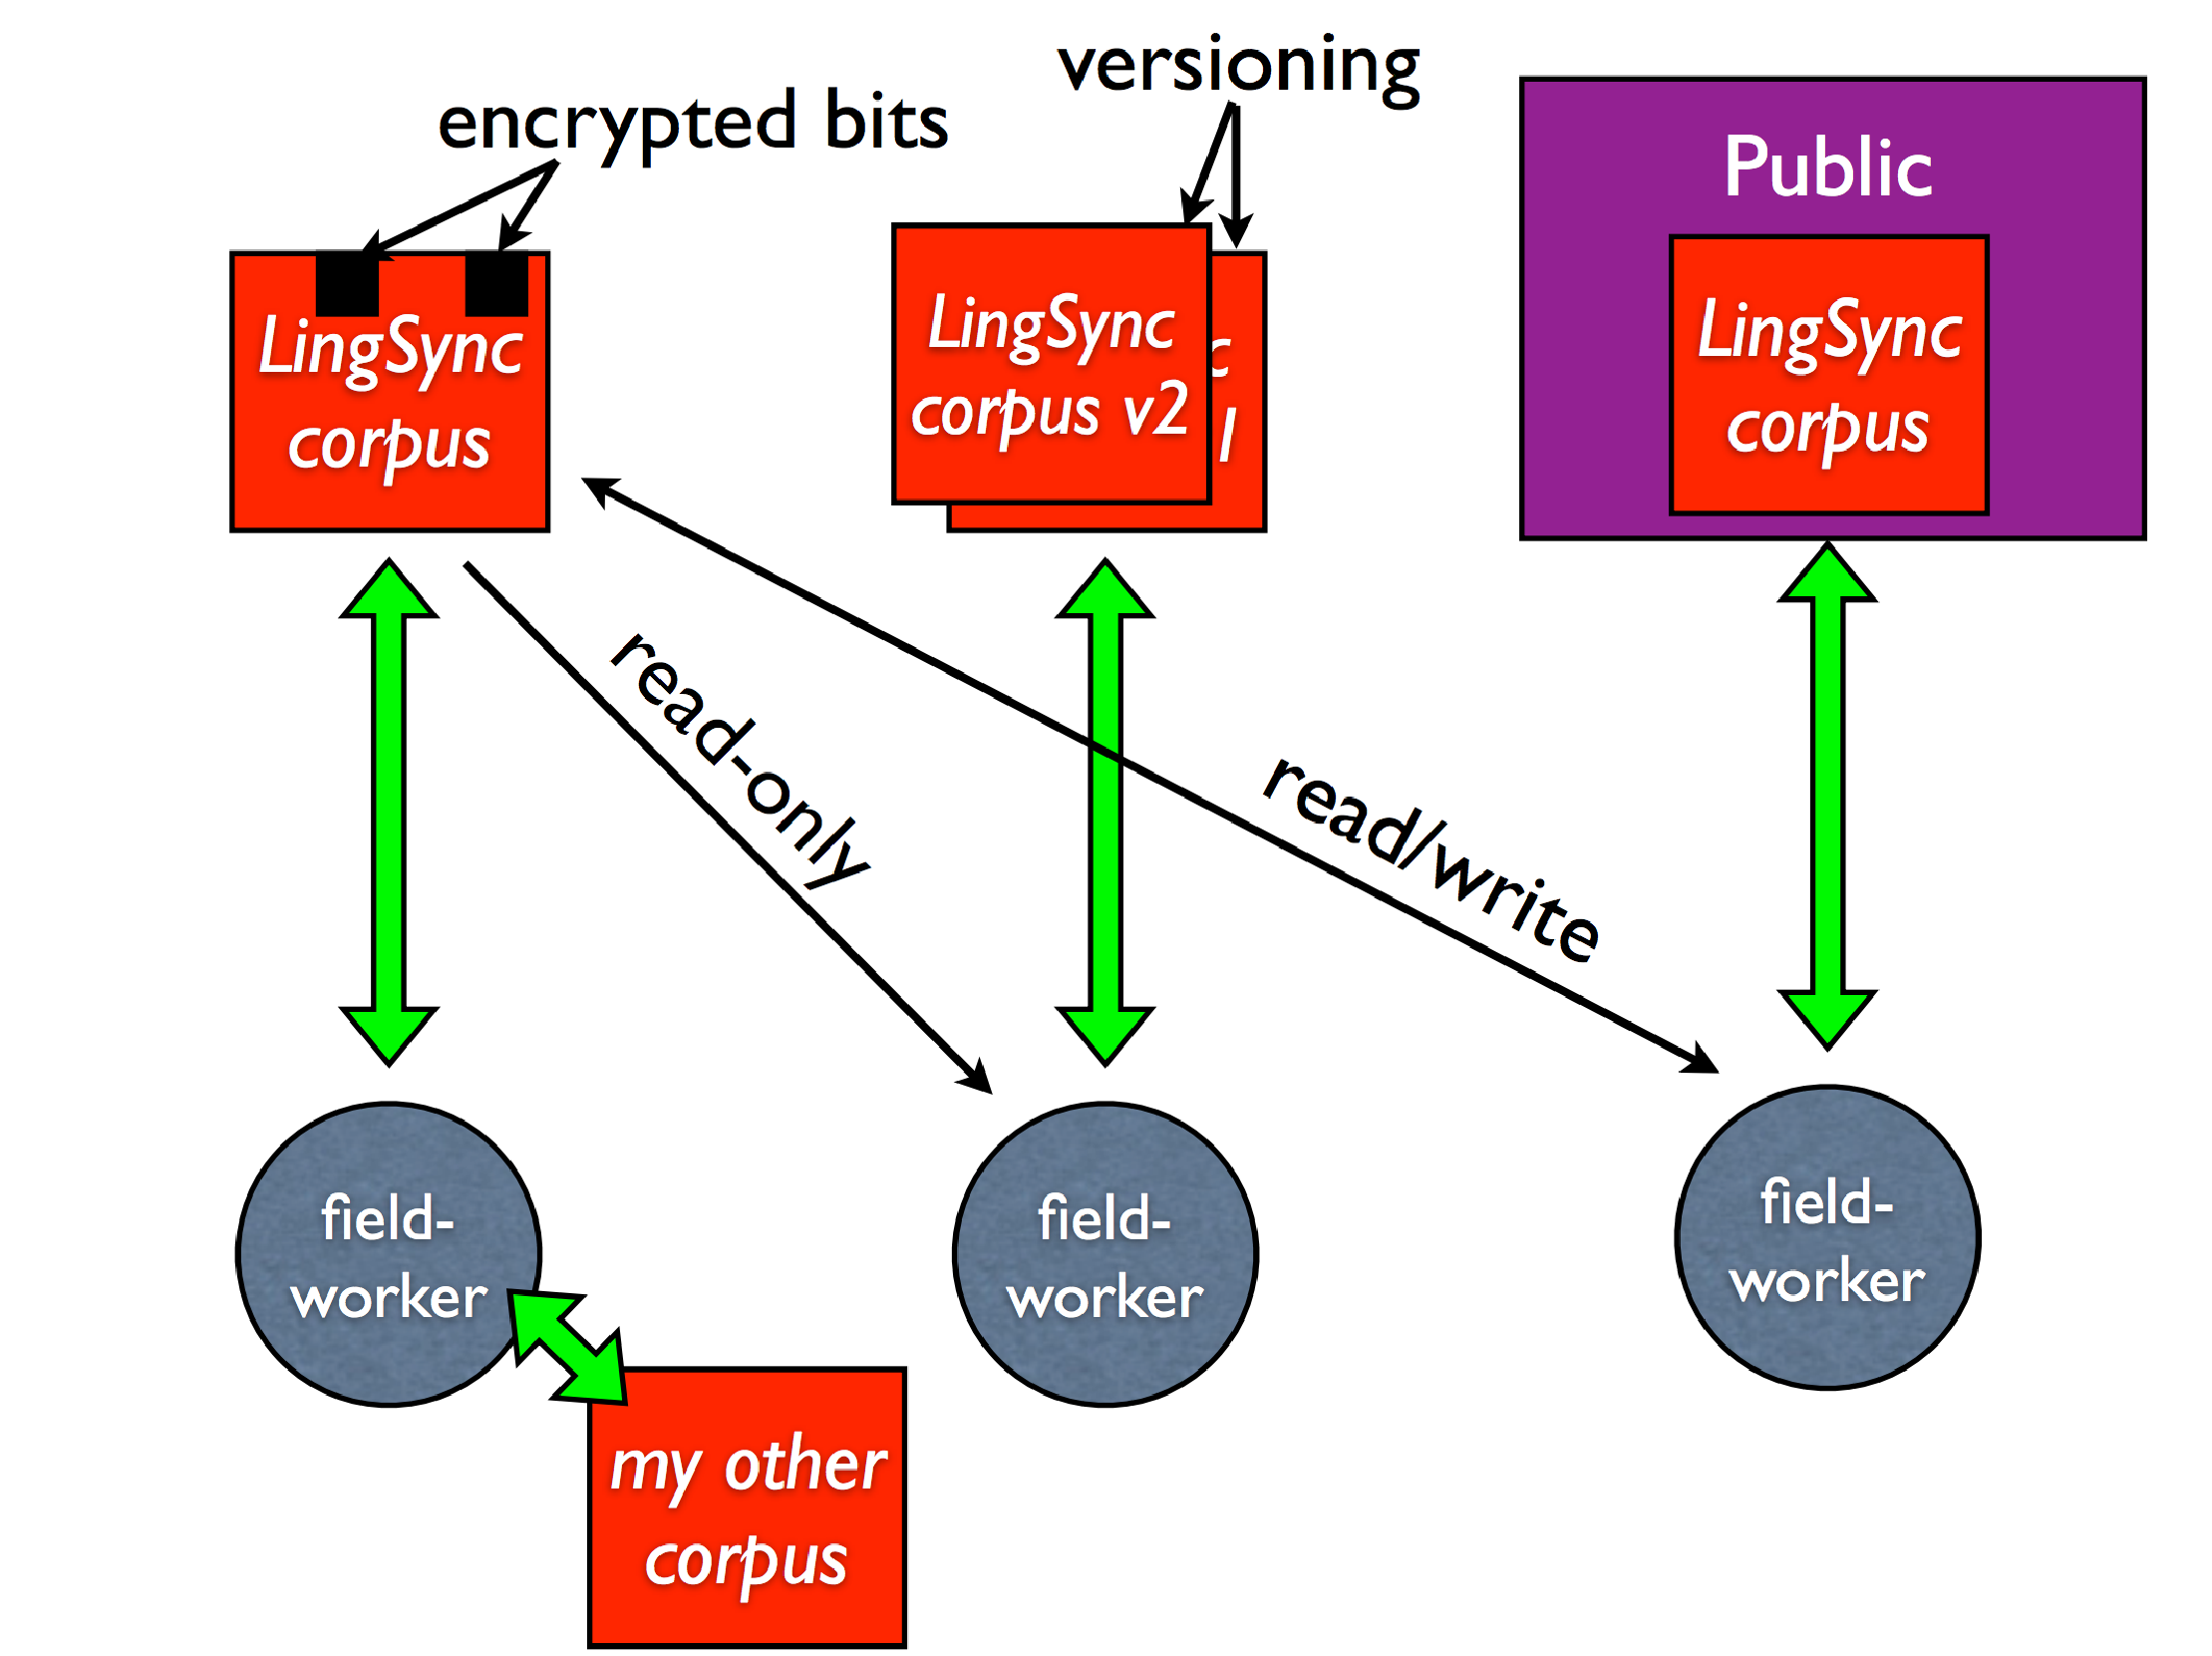
\includegraphics[width=3in]{../figures/corpora}
\label{lingsync:corpora}
\end{center}
\end{figure}

\note[item]<1>{A user can create any number of corpora. They
    may grant access at various levels to any one of his/her corpora. A
    corpus may also be made public so that it can be accessed without
    password-based authentication.}
\note[item]<1>{Portions of a corpus can be encrypted at a fine-grained level
    if that kind of control over access is required.}
\note[item]<1>{Finally, all data has version numbers which means that changes can be undone and are 
    traceable to cleaning scripts or humans who made the changes. Clearly,
    this is an important feature in the context of collaborative data creation.}

%\note[item]<2>{The OLD architecture is similar to that of LingSync in many respects}
%\note[item]<2>{Without going into too much detail, the major architectural
%    difference between the two systems is that in a language-specific OLD application users 
%    contribute to a single repository of language data to which all other users, by default,
%    have access; in contrast, LingSync, as mentioned above, assumes allows users
%    to create private corpora that they can grant various levels of access to.
%    %Essentially, the OLD assumes more data-sharing from the offset while LingSync assumes
%    % smaller teams of collaborators who can open subsets of their data as desired.
%}

\end{frame}

%\subsection{OLD}\label{sec:old}


%\subsection{LingSync/OLD}

\subsection[Data Structure]{Generality in Data Structure}\label{sec:generality}

\begin{frame}
\frametitle{Generality in data structure}
\begin{itemize}
    \item FLEx, Toolbox, etc.
        \begin{itemize}
            \item lexical entry is primary
            \item Boasian trilogy: texts, grammar, and dictionary
        \end{itemize}
    \item LingSync and OLD
        \begin{itemize}
            \item datum/form is primary
            \item elicitations, corpora, texts, grammar, dictionary, handouts, language lessons
        \end{itemize}
\end{itemize}
\note[item]<1>{The data structures assumed by LingSync and the OLD
    are arguably more general than those of similar applications like FLEx and
    Toolbox.}
\note[item]<1>{This greater generality allows these tools to be useful to a wider
    range of fieldworkers.}
\note[item]<1>{The fundamental unit of data is
    something quite unconstrained which in LingSync is called a "datum" and in
    the OLD is called a "form".}
\note[item]<1>{This abstract data unit may be used to represent sentences, phrases,
    words, or morphemes.}
\note[item]<1>{Texts, corpora, and records of elicitation sessions can then be
    constructed as (possibly ordered) sets of these data points.}
\note[item]<1>{Similarly, grammars can be created as texts which embed via reference
    these data points. And dictionaries could be constructed from these units as
    well.}
\note[item]<2>{This contrasts with the data structures that underpin FLEx and
    Toolbox; these tools assume that a grammar and a dictionary with supporting
    texts are the ultimate goals of the fieldworkers who use them. However,
    this is not always the case.}

\end{frame}


\subsection{User adoption}

\begin{frame}
\frametitle{User Adoption}
\begin{table}[h]
\begin{center}
\scriptsize
\begin{tabular}{lrrrr}
      \toprule
                     ~ &  Active & Investigating & In-active & Total\\
      \midrule
      Public Corpora  &       2 &   1 &   2 & 5 \\ 
      Private Corpora &      15 &  37 & 321 & 373\\ 
      Users           &      38 &  43 & 220 & 301 \\
      Documents & 13,408 & 2,763 & 4,541 &23,487\\
      Disk Size & 1GB & .9GB & 5.3GB& 7.2GB\\
      
      \bottomrule

\end{tabular}
\caption{Data in LingSync corpora (Feb 14, 2014). Active corpora: $>$300
activities; Investigating corpora: 300-10 activities; Active users: $>$100
activities; Investigating users: 100-10 activities.}
\label{lingsync-data}
 \end{center}
 \normalsize
\end{table}

\note[item]{There are, in total, some 300 users, 400 corpora and 24,000
    documents, i.e., the general-purpose data points mentioned above.}
\end{frame}


\begin{frame}

\begin{table}[h]
 \begin{center}
     \scriptsize
\begin{tabular}{lrrrrr}

      \toprule
      language &                     \emph{forms}  & texts & audio & GB   & speakers \\
      \midrule
      Blackfoot (\textit{bla}) &     8,847  & 171   & 2,057 & 3.8  & 3,350    \\ % 11,075 4047074461 bytes
      Nata (\textit{ntk}) &          3,219  & 32    & 0     & 0    & 36,000   \\ % 3,251  0 bytes
      Gitksan (\textit{git}) &       2,174  & 6     & 36    & 3.5  & 930      \\ % 2,216  3787227136 bytes
      Okanagan (\textit{oka}) &      1,798  & 39    & 87    & 0.3  & 770      \\ % 1,924  349478912 bytes
      Tlingit (\textit{tli}) &       1,521  & 32    & 107   & 12   & 630      \\ % 1,660  12906459136 bytes
      Plains Cree (\textit{crk}) &   686    & 10    & 0     & 0    & 260      \\ % 696    0 bytes
      Ktunaxa (\textit{kut}) &       467    & 33    & 112   & 0.2  & 106      \\ % 612    176128000 bytes
      Coeur d'Alene (\textit{crd}) & 377    & 0     & 199   & 0.0  & 2        \\ % 576    28659712 bytes
      Kwak'wala (\textit{kwk}) &     98     & 1     & 1     & 0.0  & 585      \\ % 100    7450624 bytes
      TOTAL &                        19,187 & 324   & 2,599 & 19.8 &         \\ % 22,110 21302477981 bytes
      \bottomrule

\end{tabular}
\caption{Data in OLD applications (Feb 14, 2014)}
\label{old-data}
 \end{center}
 \normalsize
\end{table}

\note[item]{Here we can see that fieldwork is being performed on nine
    endangered and/or under-documented languages using the OLD software.}
\note[item]{The languages that have seen the most use are Blackfoot,
    Nata, Gitksan, Okanagan, and Tlingit.}
\note[item]{The speaker population figures in the rightmost column are
    from Ethnologue and are probably optimistic or out-of-date. In any
    cases, most of these languages are endangered to highly endangered.}
\note[item]{We claim that these usage statistics indicate that field workers are actively 
  seeking new tools like LingSync and the OLD.}

\end{frame}

%\section[Data]{Using LingSync/OLD}\label{open-data}
%
%\begin{frame}
%Using LingSync/OLD
%\end{frame}


\section[Plugins]{Plugins \& Reusing existing tools and libraries}

\subsection{Audio}
%\subsubsection[Alignment]{Audio-transcription alignment}
%
%\begin{frame}
%
%\begin{figure}
%\begin{center}
%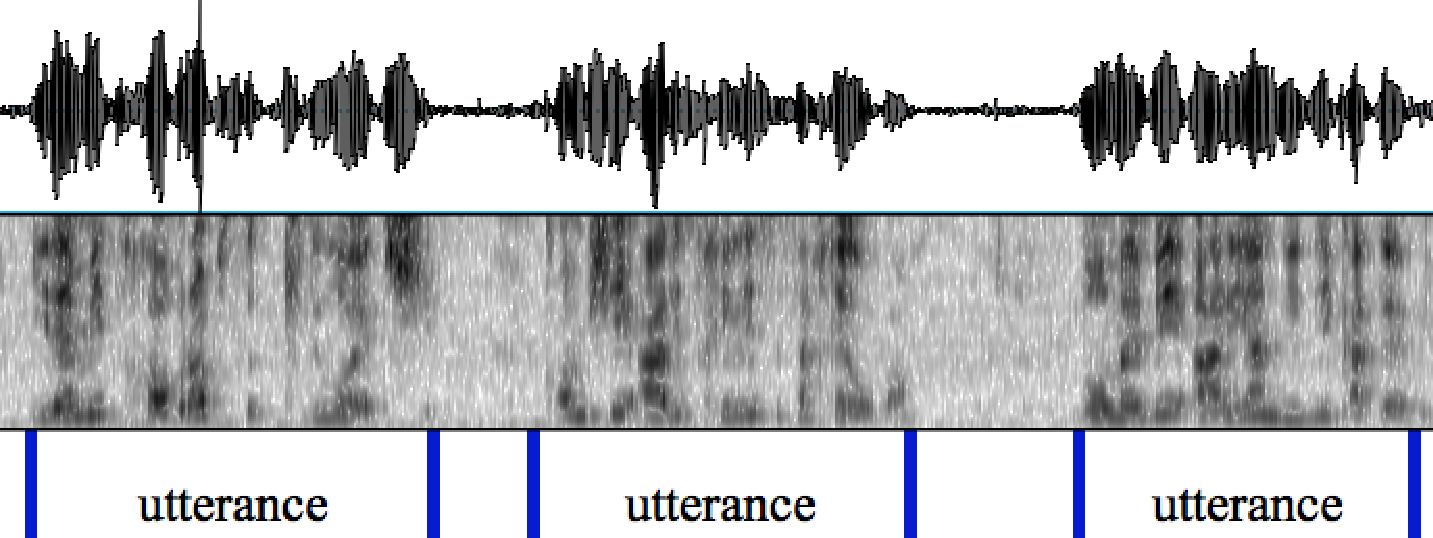
\includegraphics[width=3in]{../figures/utterance_extraction}
%\caption{Screenshot of the utterance extraction process which converts any
%audio/video into utterance intervals encoded either as \gls{json} or TextGrid using
%the PraatTextGridJS library.}
%\label{utterance_extraction_screenshot}
%\end{center}
%\end{figure}
%
%
%\note{Josh/Gina presents}
%\end{frame}




\begin{frame}
\frametitle{Plugins}
\begin{itemize}
	\item Audio
	\item Lexicon
\end{itemize}

\note{In this section I will show some screenshots of a couple of our more interesting plugins for~\\~ \\audio processing and\\lexicon visualization.}
\end{frame}

\subsubsection[ASR]{Speech Recognition for Information Retrieval}

\begin{frame}
\frametitle{Kartuli Speech Recognizer}
\begin{figure}
\begin{center}
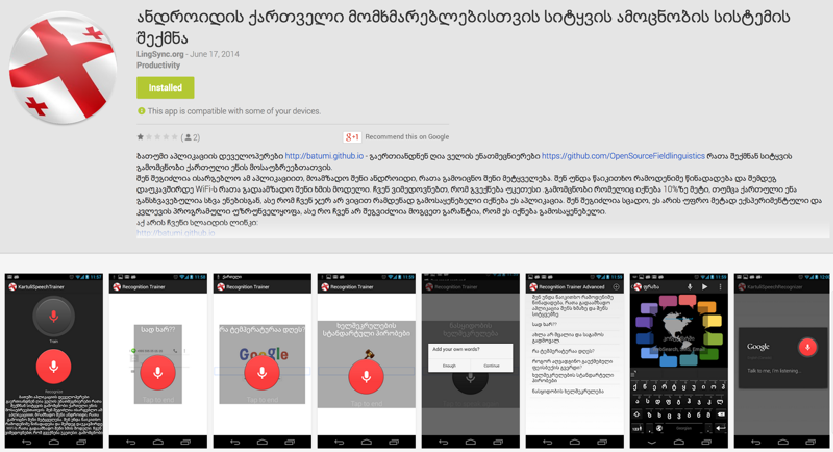
\includegraphics[width=3in]{../figures/kartuli_speech_recognition}
\caption{Screenshot of the Speech Recognition trainer}
\label{speech_recognition_screenshot}
\end{center}
\end{figure}
\note[item]{The Android speech recognition app is an app which is available on Google play for Kartuli speakers.}
\note[item]{It was built last semester while I was in the field in Batumi.}
\note[item]{The app uses the Learn X interface to permit users to train it to to their voice and vocabulary.}
\note[item]{The sentences the users say become datum in their private corpus which is in turn used to re-train their own personal language model.}
\note[item]{If you would like to see it in action you can download it from the Play store, (search for Kartuli speech recognizer) or come see us at the demos later.}
\note[item]{We dont expect recognition rates better than 10\% but we are hoping by letting users import their SMS or other text on their Android it will be come personalized enough to recognize their own speech in limited contexts such as SMS messages. }
\end{frame}


\subsection{Morphology}



%\subsubsection[Existing]{Existing morphological parsers}
%
%\begin{frame}
%
%\begin{figure}
%\begin{center}
%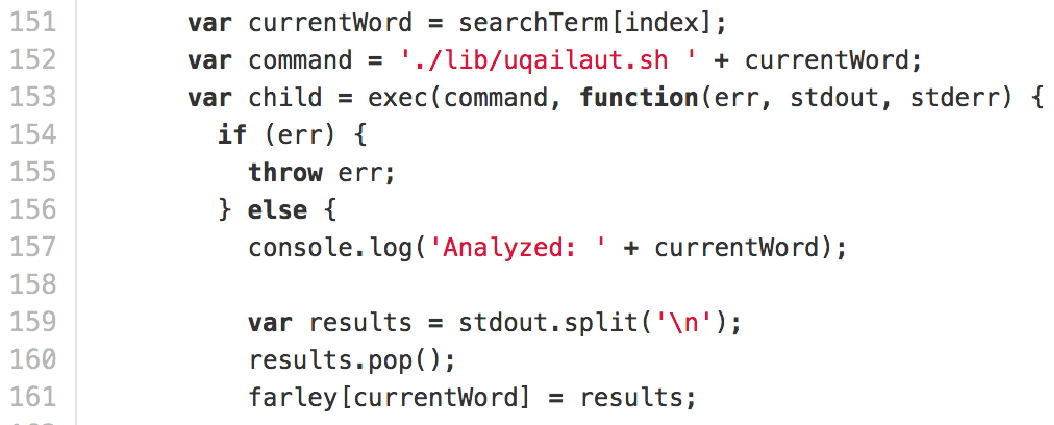
\includegraphics[width=2.5in]{../figures/farley} 
%\\
%\includegraphics[width=2.5in]{../figures/inuktitut}
%\caption{Screenshot of Farley's Morphological Analyzer wrapped in a Node.js Web Service And offered in a HTML5 User Interface  }
%\label{speech_recognition_screenshot}
%\end{center}
%\end{figure}
%%\hspace{3in}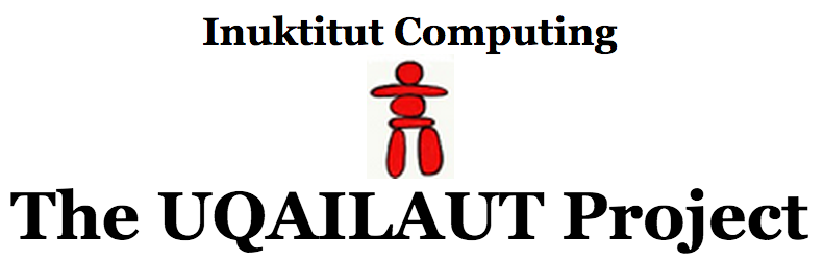
\includegraphics[width=1in]{../figures/inuktitut_computing}
%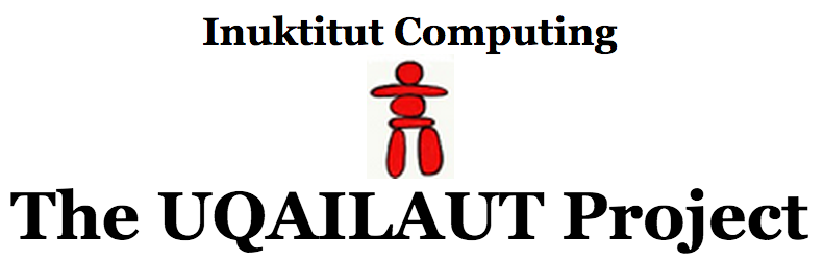
\includegraphics[width=1in]{../figures/inuktitut_computing}

%\note{Josh/Gina presents}
%\end{frame}




\subsubsection[DataViz]{Data Visualizations}

\begin{frame}

\frametitle{\large Force directed graph of morphemes in context}

\begin{figure}
\begin{center}
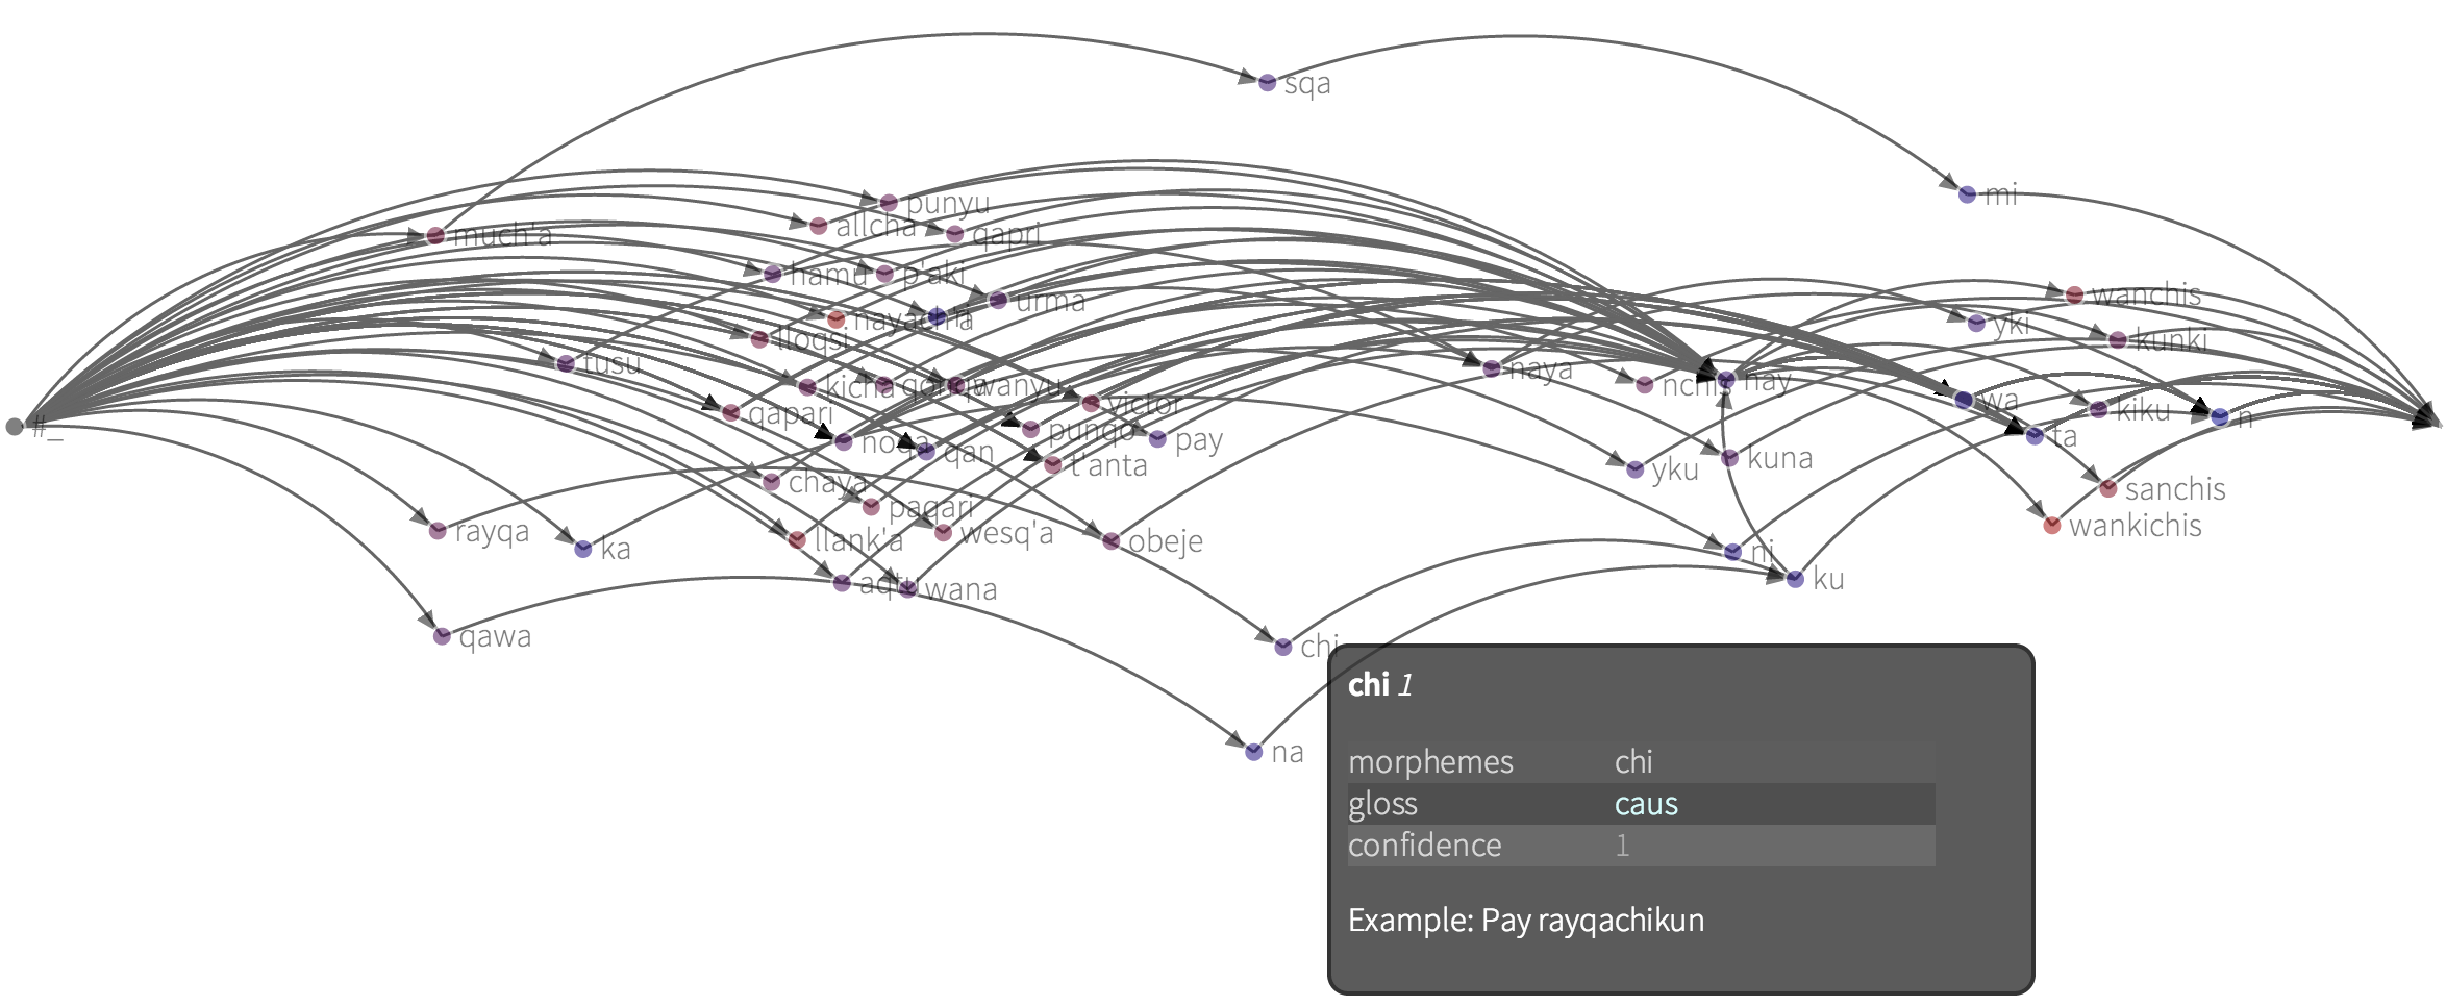
\includegraphics[width=4in]{../figures/lexicon_browser}
\label{lexicon_graph_screenshot}
\end{center}
\end{figure}

\note[item]{This visualization lets you see precendence order of morphemes in your corpus in a connected graph}
\note[item]{The node on the left is the beginning of the word and the node on the right is the end of the word.}
\note[item]{You can also choose not to plot the end nodes, and then you can see if the corpus has a focus on one morpheme. This data here is from M.E. dissertation about the interactions of the morpheme's -naya and -ta in Cusco Quechua, and this can be seen as they are the focal points of the graph.}
\end{frame}


\begin{frame}
\frametitle{\large WordCloud showing words by frequency}
\begin{figure}
\begin{center}
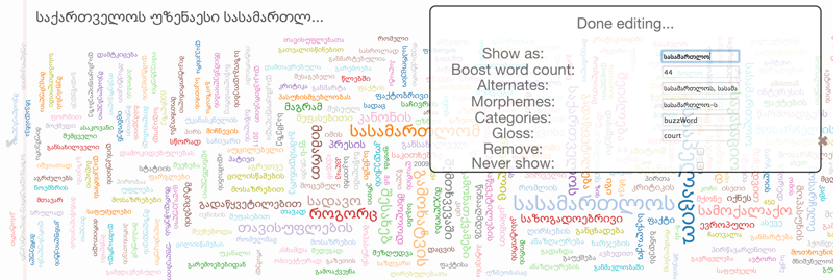
\includegraphics[width=4in]{../figures/lexicon_browser2}
\label{lexicon_frequency_screenshot}
\end{center}
\end{figure}

\note[item]{The second visualization is a word cloud visualization which Josh built using Jason Davies' D3 word cloud  layout engine.}
\note[item]{Unlike Wordle, it runs in Javascript (not a Java applet) and so it works on iPads, Androids and all browsers.}
\note[item]{While it's not as beautiful as Wordle, it  supports the full unicode character set.}
\note[item]{We added some logic for language independent automatic detection of function words (stop words) and tokenization.}
\note[item]{My language consultants use this to clean head words, add segmentation, gloss or other lexical information. They get visual feedback in that the content-ful words begin to pop out as they clean, and the cloud becomes more representative of the meaning of the document.}
\note[item]{The app is on Google Play and on the Chrome Store, search for iLanguage Cloud or come see us at the demos.}
\end{frame}




\subsubsection[Blackfoot]{OLD morphological parsers (Blackfoot)}

\begin{frame}
\frametitle{OLD morphological parsers (Blackfoot)}
Goals
\begin{itemize}
    \item Present and motivate the OLD's approach to creating morphological parsers
    \item Demonstrate the use of this functionality via two Blackfoot parsers
\end{itemize}
\note[item]{Now I'd like to discuss the OLD's morphological parser functionality. I
    will present and motivate the OLD's approach to creating morphological
    parsers with reference to two parsers created for Blackfoot, an endangered
    language which is from the Algonquian language family and which is spoken
    in Alberta, Canada and Montana, USA.}
\note[item]{This portion of our presentation should segue nicely into the next talk
    which discusses a similar but interestingly different approach to modelling
    the morphology and phonology of another endangered Algonquian language: Plains Cree.}
\end{frame}


\begin{frame}
\frametitle{OLD Morphological Parsers}
Requirements (fieldworkers should be able to):
\note[item]<1>{Here are the requirements that guided the design of the OLD's
    functionality for creating morphological parsers}
\begin{itemize}
    \item create parsers that
        \begin{itemize}
            \item<1->are practical and forgiving
                \note[item]<1>{Fieldworkers should be able to create
                    morphological parsers that are practical and forgiving.  By
                    \textit{practical} I mean that they should be able to
                    suggest correct, or largely correct, word analyses during
                    data entry. By \textit{forgiving} I mean that I want
                    fieldworkers to be able to create parsers without first
                    having a full and perfect analysis of the morphophonology
                    of their language of study.}
            \item<2->make use of existing fieldworker skills
                \note[item]<2>{Since fieldworkers are being encouraged to create
                    their own parsers, they should be able to do so by making use
                    of the skills that they already have. That is, they should not
                    be required to first learn wholly unfamiliar formalisms.}
            \item<3->make use of data in the system
                \note[item]<3>{Fieldworkers should be able to build parsers
                    using the expertly analyzed data that already exist in their
                    databases; for example, morphologically analyzed words in
                    IGT format and categorized and phonemically transcribed
                    lexical entries.}
            \item<4->are tailored to a specific purpose
                \note[item]<4>{Fieldworkers should be able to create different
                    parsers for different purposes. Examples include orthographic
                    parsers which parse orthographic transcriptions and phonetic
                    parsers which parse phonetic transcriptions. It should also
                    be possible to tailor phonetic parsers to the grammars of
                    individual speakers or dialects. Fieldworkers should also
                    be able to create analysis-specific variants of all of
                    these.}
            \item<5->facilitate automated analysis testing
                \note[item]<5>{Since the parsers are comprised of computational
                    implementations of analyses and models of the lexicon,
                    morphology, and phonology, they should facilitate the
                    automated testing of these analyses and models against
                    specified data sets in the system.}
            \item<6->are reusable: spell-checkers, pronunciation dictionaries, \ldots
                \note[item]<6>{The components of the parsers should be reusable for,
                    say, the creation of spell-checkers or the generation of
                    pronunciation dictionaries that can be used in
                    audio-transcription aligners.}
        \end{itemize}
\end{itemize}
\end{frame}


\begin{frame}
\frametitle{OLD Morphological Parsers}
\begin{figure}
\begin{center}
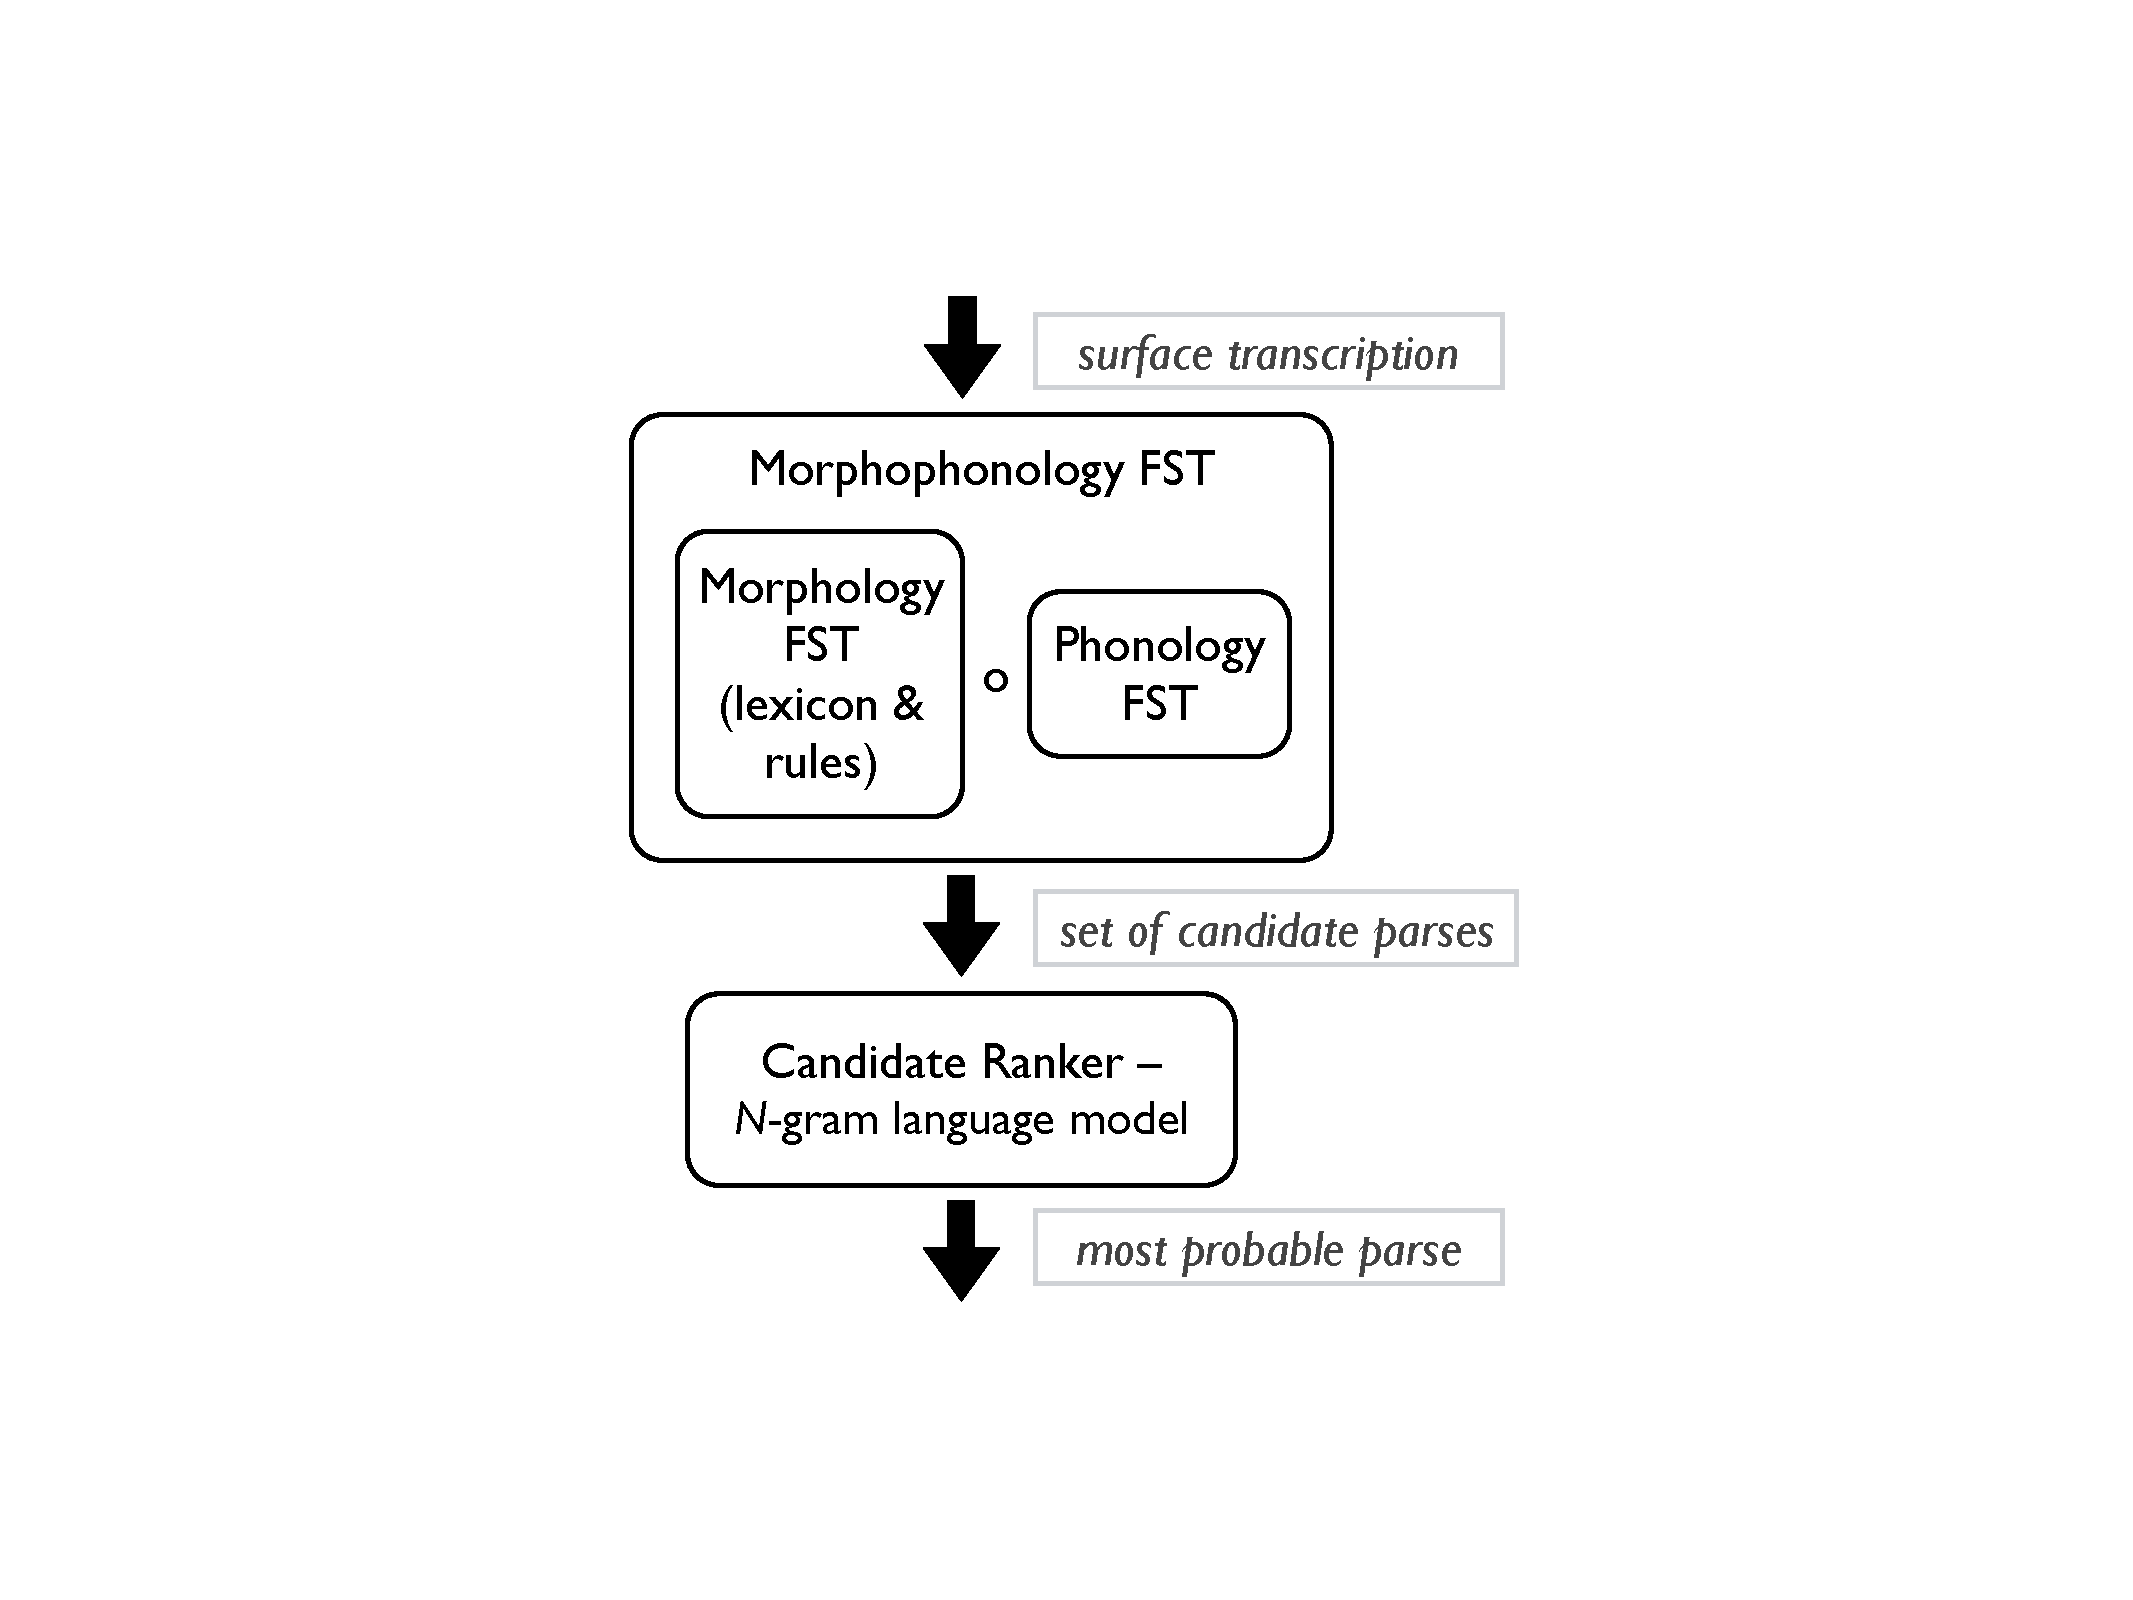
\includegraphics[width=0.6\textwidth]{../figures/OLD-parser-diagram-2}
\caption{Architecture of an OLD morphological parser.}
\label{fig:arch}
\end{center}
\end{figure}
\note[item]{This diagram provides a high-level overview of the components of an
    OLD morphological parser.}
\note[item]{The morphophonology is a finite-state transducer that takes a
    surface transcription as input and returns a set of candidate parses as
    output; it is the composition of a phonology transducer and a morphology
    transducer.}
\note[item]{The candidate ranker assigns a probability to each candidate parse 
    returned by the morphophonology; it is built upon an $N$-gram language
    model.}
\end{frame}


%\begin{frame}
%\frametitle{OLD Phonologies}
%\begin{itemize}
    %\item<1->A transducer wholly defined by the fieldworker as ordered
        %context-sensitive rewrite rules \`{a} la SPE
%\end{itemize}
%\note[item]{The phonology FST specifies phonological transformations or spelling
%rules; \textit{It is completely specified by the fieldworker} as an ordered
%list of context-sensitive rewrite rules using the regular expression rewrite
%rule syntax accepted by foma and Xerox FST}
%\note[item]{The morphology recognizes sequences of morphemes that correspond to
%grammatical words. A morphology is constructed by the system using data
%extracted from two OLD corpora that are created and specified by the
%fieldworker. From the one corpus are extracted lexical items, i.e.,
%morphemes. From the other corpus are extracted the sequences of categories
%that constitute the morphotactic rules.}
%\note[item]{The LM is estimated by the OLD based on the analyzed words in a
%corpus created and specified by the fieldworker.}
%\end{frame}

\begin{frame}[fragile]
\frametitle{OLD Phonologies}

\begin{itemize}
    \item<1->Phonology: a transducer wholly defined by the fieldworker as ordered
        context-sensitive rewrite rules
        \note[item]<1>{An OLD phonology is a transducer that is defined explicitly
            and in its entirety by the fieldworker as an ordered list of
            context-sensitive rewrite rules.}
\end{itemize}

\begin{uncoverenv}<2->
\ex<nitsspiyi> /nit-ihpiyi/ $\rightarrow$ $<$nitsspiyi$>$\xe
\end{uncoverenv}
\note[item]<2>{Example (\getref{nitsspiyi}) shows a Blackfoot word segmented
    into phonemically transcribed morphemes and its phonetico-orthographic
    surface representation.}

\vspace{-1cm}

\begin{uncoverenv}<3->
\ex<phonology>\verb+define phonology [+\\
\verb+    [ "-" -> s || t _ i ] .o.+\\
\verb+    [ i h -> s || s _ ] ] ;+\\
\verb+#test nit-ihpiyi -> nitsspiyi+
\xe
\end{uncoverenv}
\note[item]<3>{(\getref{phonology}) shows the definition of a simple phonology
    FST that implements the mapping in (\getref{nitsspiyi}).}
\note[item]<3>{The phonology is written in the regular expression rewrite rule
    language that is accepted by FST toolkits like foma and Xerox's XFST.}

\vspace{-0.5cm}

\begin{itemize}
    \item<4->make use of existing fieldworker skills
        \note[item]<4>{Since these rewrite rules are simply notational variants of
            the SPE-style rewrite rules that most linguistic fieldworkers are
            familiar with, the system makes use of existing fieldworker skills.}
        \note[item]<4>{The second line in (\getref{phonology}), for example, is
            a rule which transforms the hyphen morpheme delimiter to an "s" when
            it occurs after a "t" and before an "i". A fieldworker can immediately
            begin using this formalism after learning a few simple notational 
            oddities, such as the use of double vertical lines in place of the
            forward slash that is customary in rule-based phonology texts.}
    \item<5->facilitate automated analysis testing
        \note[item]<5>{Also, since the fieldworker has full control over the
            definition of phonological transformations (or spelling rules),
            they can use the functionality to test their analyses of this
            component of the grammar. For example, the parser can be used to
            automate the discovery of words in the database that its
            morphophonology cannot analyze; This may lead to modifications of
            the underlying analyses and models.}
        \note[item]<5>{One restricted but useful example of automated analysis
            testing is provided by the phonology test comment beneath the
            phonology definition. The left side of the arrow is the underlying
            representation and the right side is the surface representation.
            The OLD recognizes these comments in FST rewrite rule scripts and
            reports back on what percentage of the tests are passed by the
            phonology. This facilitates test-driven phonology development.}
\end{itemize}

\end{frame}


\begin{frame}
\frametitle{OLD Morphologies and Morpheme LMs}
\ex<danced>
\begingl
\gla Nitsspiyi //
\glb nit-ihpiyi //
\glb 1-dance //
\glb agra-vai //
\glft 'I danced.' //
\endgl
\xe
\note[item]<1>{OLD applications are full of morphologically analyzed
words like the Blackfoot one in (\getref{danced}).}

\vspace{-1cm}

\begin{uncoverenv}<2->
%\ex<mtactic>W $\rightarrow$ AGR - VAI\\AGR $\rightarrow$ \textit{nit}\\VAI $\rightarrow$ \textit{ihpiyi}\xe
\ex<mtactic>\begin{tabular}{lll}
w & $\rightarrow$ & agr - vai \\
agr & $\rightarrow$ & \emph{nit} \\
vai & $\rightarrow$ & \emph{ihpiyi} \\
\end{tabular}\xe
\end{uncoverenv}
\note[item]<2>{(\getref{mtactic}) is a rewrite rule representation of the
    morphological generalizations that can be extracted from a corpus of forms
    like (\getref{danced}) and implemented as an FST, in either the Lexicon
    Compiler (lexc) or Regular Expression Rewrite Rule (regex) language.}
\note[item]<2>{Note that the OLD does not currently allow users fine-grained
    control over morphology specification. That is, it is not currently
    possible to use flag diacritics to implement long-distance dependencies as
    illustrated by Snoek et al. in the precedings of this workshop. Of course,
    the OLD interface could easily be modified to allow users complete control
    over morphologies, perhaps with the option of using the system-generated
    lexical and morphotactic generalizations as a starting point.}

\vspace{-1cm}

\begin{uncoverenv}<3->
\ex<lm>\begin{tabular}{lll}
<s> & nit & ihpiyi \\
nit & ihpiyi & </s> \\
\end{tabular}\xe
\end{uncoverenv}
\note[item]<3>{(\getref{lm}) shows the morpheme trigrams that can be extracted
from a corpus of IGT forms like (\getref{danced}).}

\vspace{-1cm}

\begin{itemize}
    \item<4->make use of data in the system
        \note[item]<4>{Since the morphology FST and the morpheme LM are
            generated by the system based on data in the database, a
            significant portion of the parser creation work is automated using
            the endangered language data present in the OLD application.}
\end{itemize}

\end{frame}


\begin{frame}
\frametitle{Blackfoot Parsers}
\begin{itemize}
    \item 2 parsers, both with identical morphologies and LMs:
        \note[item]<1>{Now I'd like to quickly discuss two Blackfoot
            parsers created using the OLD morphological parser functionality.}
        \note[item]<1>{They have identical morphologies and morpheme language models.}
        \begin{itemize}
            \item<2-> lexical items from standard dictionary (Frantz 1995)
                \note[item]<2>{The lexica of these parsers are the morphemes
                    present in the standard dictionary of the language, Frantz
                    and Russell's Blackfoot Dictionary of Stems, Roots, and
                    Affixes.}
            \item<3-> morphotactic rules extracted from 3,414 well analyzed
                words types (BLA OLD)
                \note[item]<3>{The morphotactic rules, that is, the set of
                    category and delimiter sequences that correspond to valid
                    words of the language, were extracted from the 3,414 well
                    analyzed word types in the Blackfoot OLD. Well analyzed
                    words are those with fieldworker-created morphological
                    analyses such that all of the morphemes used have lexical
                    entries in the database.}
            \item<4-> morpheme LM estimated from 3,425 gold standard well
                analyzed words (BLA OLD)
                \note[item]<4>{The morpheme language models were estimated
                    based on counts from the set of well analyzed words in the
                    database such that a single best analysis can be
                    identified. This is the gold standard used for both LM creation
                    and evaluation. Each parser was created five times with a
                    different randomly sampled 90\% training set and overall
                    parser performance was tested against the corresponding
                    10\% test set.}
        \end{itemize}
    \item<5->Parser 1: phonological rules and allomorphic alternations from
        grammar (Frantz 1997)
        \note[item]<5>{The two parsers differ in their phonologies. Parser 1
            has a phonology which implements, as faithfully as I could manage,
            the general phonological rules of the grammar and the lexically
            conditioned allomorphic alternations described in that same text.}
    \item<6->Parser 2: Parser 1's phonology with length and prominence
        contrasts removed during generation; massively over-analyzes
        \note[item]<6>{Parser 2 is an attempt to improve on Parser 1 by
            modifying the phonology so that it recognizes many more surface
            forms. During generation, this phonology maps long segments to
            their short counterparts and de-accents accented characters.
            Orthographically transcribed words must be de-accented and
            de-lengthened prior to parsing attempts.}
\end{itemize}
\end{frame}

%6,592 well analyzed word tokens
%3,414 well analyzed word types
%3,425 well gold standard well analyzed word types


\begin{frame}
\frametitle{Blackfoot Parser \char"2012{} Results}
\begin{table}[t]
\centering
\footnotesize
\begin{tabular}{llllllll}
\toprule
parser & succ. & F-score & prec. & rec. & phon. & morphon. & LM \\
\midrule
1      & 0.14       & 0.32    & 0.53      & 0.23   & 0.21      & 0.20    & 0.72 \\
2      & 0.17       & 0.40    & 0.40      & 0.39   & 0.60      & 0.60    & 0.28 \\
\bottomrule
\end{tabular}
\normalsize
\caption{Blackfoot OLD morphological parser results.}
\label{tab:p2-results}
\end{table}

\note[item]<1>{This table summarizes the results of evaluating these parsers.}
\note[item]<1>{While neither has a very impressive overall success rate---14\% and
    17\%, respectively---their F-scores show that they will be practical in
    expediting the creation of IGT representations. With a GUI that presents
    a ranked list of parses during data entry, fieldworker-contributors will
    be able to edit auto-generated parses that contain, roughly and on average,
    half of the correct morphemes.}
\note[item]<1>{Also, the morphophonology transducer of Parser 2 is 60\%
    accurate, meaning that 60\% of the time the correct analysis is in the
    candidate set that it returns.  Therefore users could scroll through the
    ranked list of candidates and choose the correct one; which would be faster
    than typing it out manually.}
\note[item]<2>{The phonology of Parser 1 has a 21\% success rate while that of
    Parser 2 has a 60\% success rate. There are two primary explanations for
    the poor performance of Parser 1's phonology, i.e., that which is faithful
    to the grammar. First, the grammar's phonology does not account for
    non-lexical prominence, i.e., accenting. Second, there is a lot of
    inconsistency in terms of orthographic transcription in this
    multi-contributor data set.}
\note[item]<3>{It is interesting that the phonology of Parser 2 performs so much
    better yet the gains in overall parse rate and F-score are not as
    significant. Parser 2 essentially puts a far greater burden on the language
    model, a burden which is too much for an LM based on counts from an extremely 
    small corpus of 3,400 words. Parser 2's morphophonology transducer produces
    approximately 1,800 analysis candidates per input word. As more well
    analyzed words are added to the database with the aid of the parsers, the
    LM will improve and, as a result, so too will the parser as a whole.}
\note[item]<4>{Of course, another means of improving overall performance would
    be to improve the performance of the phonology without causing it to 
    massively overgenerate during analysis and put such a burden on the LM,
    that is, by using fieldworker knowledge to write a phonology that can
    predict the location of accented vowels. This is in the works.}

\end{frame}

\begin{frame}
\frametitle{OLD Morphological Parsers \char"2012{} Discussion}

OLD parsers exemplify a particular set of principles for guiding
computationally-assisted endangered languages fieldwork:
\note[item]<1>{The OLD approach to creating morphological parsers illustrates
    some general strategies that I would like to advocate in terms of
    computationally-assisted fieldwork on endangered languages.}

\begin{itemize}
    \item<2->exploit both fieldworker expertise and automated methods of
        grammar induction
        \note[item]<2>{We need systems that can both make use of the expertise
            of the fieldworkers who are creating these data sets, while also
            helping them to bootstrap the process with statistical and machine
            learning techniques. This is interestingly different from NLP where
            the overarching requirement would seem to be the production of
            results with as little expert guidance as one can get away with.}
        \note[item]<2>{By allowing fieldworkers real control over the
            specification of models, we not only make use of that skill set, we
            also make it easier for them to automate the testing of their
            analyses, and thereby to improve those analyses.}
        \note[item]<2>{At the same time, we should be forgiving, i.e., we
            should not REQUIRE a complete mastery of components of the grammar
            prior to the creation of useful features like automatic
            morphological analyzers.}
        \item<3->use familiar representations:
            \begin{itemize}
                \item yes: (nit-ihpiyi, 1-dance, agra-vai)
                \item no: ihpiyi+1+SG+PST
            \end{itemize}
        \note[item]<3>{We should also create systems that make use of representations
            that are familiar to fieldworkers. This has already been mentioned with
            respect to SPE-style context-sensitive rewrite rules in the specification
            of phonologies. Another example of this, however, can be seen in the
            fact that OLD parsers return morphological analyses in IGT format, i.e.,
        a morpheme segmentation line, a gloss line, and a category line.}
    \item<4->allow for multiple models
        \note[item]<4>{We need to also enable fieldworkers to implement different
            models for different purposes. In some situations, prescriptive models
            are needed such as orthographic parsers that can parse orthographic
            transcriptions and which can be used, for example, in the creation of
            spell-checkers. In other situations, descriptive models of various types
            are needed. For example, speaker-, dialect-, and/or analysis-specific
            models that can analyze and generate phonetic representations and which
            can be used to test analyses and, for example, to create
            pronunciation dictionaries for audio-to-text alignment tools.}
\end{itemize}
\end{frame}

%facilitate the creation of practical parsers (forgiving)

%are practical and forgiving
%make use of existing fieldworker skills
%make use of data in the system
%are tailored to a specific purpose
%facilitate automated analysis testing
%are reusable: spell-checkers, pronunciation dictionaries,


\section{The Take-Home}

\begin{frame}
\frametitle{Take Homes}
\begin{itemize}
    \item Finding effective tools for fieldwork on endangered languages is non-trivial
    \item All stakeholders, All devices
    %\item High productivitiy requirements
    \item Modular Web Services and Plugin Architecture 
    \item Open Source, Open Development, Open Data 
    \item Providing glue for fieldworkers and computational linguists to collaborate
\end{itemize}

\note[item]{We hoped to demonstrate that finding tools for fieldwork for endangered languages is not trivial  task.}
\note[item]{We wanted to include all stakeholders and all devices}
\note[item]{The way we achieved this was by using modular web services and a plugin architecture}
\note[item]{Everything is open source, our development is open which means you can see all the features and requests as well as completed milestones and future milestones. we enable open data but do not enforce it}
\note[item]{We provide the glue for field workers and computational linguists to collaborate without becoming frustrated or feeling like they are loosing precious time which could be used to further their own research programs.}
\end{frame}

\section*{(Our Team)}

\begin{frame}
\frametitle{Acknowledgements}

\small
Tobin Skinner, Elise McClay, Louisa Bielig, MaryEllen Cathcart, Theresa
Deering, Yuliya Manyakina, Gretchen McCulloch, Hisako Noguchi, Brian Doherty,
Gay Hazan, Oriana Kilbourn, Kim Dan Nguyen, Rakshit Majithiya, Mietta Lennes,
Nivja de Jong, Ton Wempe, Kyle Gorman, Curtis Mesher, Beso Beridze, Tornike
Lasuridze, Zviadi Beradze, Rezo Turmanidze, Jason Smith, Martin Gausby, Pablo
Duboue, Xianli Sun, James Crippen, Michael McAuliffe, Patrick Littell, Faryal
Abbasi, Farah Abbasi, Tamila Paghava, Esma Chkhikvadze, Nina Gatenadze, and
Mari Mgeladze, Jessica Coon, Alan Bale, Michael Wagner, Henry Davis, Lisa
Matthewson, Alexandre Bouchard-Côté
~\\
~\\
SSHRC Connection Grant (\#611-2012-0001) \\
SSHRC Standard Research Grant (\#410-2011-2401) \\
SSHRC Image, Text, Sound \& Technology (\#849-2009-0056)
\normalsize
\note{We would like to thank our linguistics student interns, computer science
    student interns and countless other open source software developers who
    directly or indirectly helped build LingSync/OLD to what it is today and
    will be in the future. \\
~\\
We would like to thank the ComputEL workshop reviewers, our users and would be
users for providing feedback, suggestions, asking tough questions, and sending
bug reports. \\
~\\
We would like to thank our language consultants for their friendship, patience
and for sharing their language with us.\\
~\\
We would also like to thank the SSHRC council for explicitly supporting "open
source approaches to knowledge mobilzation." }

\end{frame}



\begin{frame}
\frametitle{References - ბიბლიოგრაფია}
\tiny
\begin{itemize}
%\item Dorothee Beermann and Pavel Mihaylov. 2012. TypeCraft collaborative databasing and resource sharing for linguists. Language Resources and Evaluation, pages 1?23.
%\item Kenneth R Beesley and Lauri Karttunen. 2003. Finitestate morphology: Xerox tools and techniques. CSLI, Stanford.
%\item H. Andrew Black and Gary F. Simons. 2006. The SIL FieldWorks Language Explorer approach to morphological parsing. In Computational Linguistics for Less-studied Languages: Proceedings of Texas Linguistics Society, Austin, TX.
%\item Lynnika Butler and Heather van Volkinburg. 2007. Review of FieldWorks Language Explorer (FLEx). Language Documentation \& Conservation, 1(1):100?106.
\item MaryEllen Cathcart, Gina Chiodo, Theresa Deering, Yuliya Manyakina, Gretchen McCulloch, and Hisako Noguchi. 2012. LingSync: A free tool for creating and maintaining a shared database for communities, linguists and language learners. In Robert Henderson and Pablo Pablo, editors, Proceedings of FAMLi II: workshop on Corpus Approaches to Mayan Linguistics 2012, pages 247-250.
%\item N. Chomsky and M. Halle. 1968. The Sound Pattern of English. Harper \& Row, New York.
\item Jonathon E. Cihlar. 2008. Database development for language documentation: A case study in the Washo language. Master's thesis, University of Chicago.
%\item Gina Chiodo. 2009. Morphological parsing of Inuktitut. Ms, Concordia University, Faculty of Engineering and Computer Science.
%\item David Costa. 2012. Surveying the sources on the Myaamia language. In Proceedings of the 2012 Myaamiaki Conference.
\item N.H. De Jong and T Wempe. 2009. Praat script to detect syllable nuclei and measure speech rate automatically. Behavior research methods, 41(2):385-390.
%\item Joel Dunham. 2014. Online Linguistic Database documentation. http://online-linguistic-database. readthedocs.org, March.
\item Joel Dunham. 2014. The Online Linguistic Database: Software for linguistic fieldwork. PhD dissertation, UBC. (\textit{To appear.})
\item Benoit Farley. 2012. The Uqailaut project. http://www.inuktitutcomputing.ca, January.
%\item http: Scott Farrar. 2010. Review of TypeCraft. Language
%\item Documentation \& Conservation, 4:6065.
%\item Donald G. Frantz and Norma Jean Russell. 1995. Blackfoot Dictionary of Stems, Roots, and Affixes. Toronto: University of Toronto Press.
%\item Donald G. Frantz. 1991. Blackfoot Grammar. Toronto: University of Toronto Press.
%\item Andrew Garrett, Juliette Blevins, Lisa Conathan, Anna Jurgensen, Herman Leung, Adrienne Mamin, Rachel Maxson, Yoram Meroz, Mary Paster, Alysoun Quinby, William Richard, Ruth Rouvier, Kevin Ryan, and Tess Woo. 2001. The Yurok language project. http://linguistics.berkeley.edu/ yurok/index.php, January.
%  \item Andrew Garrett, Susan Gehr, Line Mikkelsen, Nicholas Baier, Kayla Carpenter, Erin Donnelly, Matthew Faytak, Kelsey Neely, Melanie Redeye, Clare Sandy, Tammy Stark, Shane Bilowitz, Anna Currey, Kouros Falati, Nina Gliozzo, Morgan Jacobs, Erik Maier, Karie Moorman, Olga Pipko, Jeff Spingeld, and Whitney White. 2009. Karuk dictionary and texts. http://linguistics.berkeley.edu/karuk/links. php, January.
%  \item Jeff Good. 2012a. Community collaboration in Africa: Experiences from northwest Cameroon. Language Documentation and Description, 11(1):2858.
  \item Jeff Good. 2012b. Valuing technology: Finding the linguists place in a new technological universe. In Louanna Furbee and Lenore Grenoble, editors, Language documentation: Practice and values, pages 111131. Benjamins, Amsterdam.
%  \item K David Harrison. 2007. When Languages Die: The Extinction of the Worlds Languages and the Erosion of Human Knowledge. Oxford University Press.
%  \item M. Hulden. 2012. foma: finite state compiler and C library (documentation). https://code.google.com/p/ foma/w/list.
%  \item George Ironstrack. 2012. Miloniteeheetaawi eehinki pimihkanaweeyankwi: Lets reflect on how far we have traveled. In Proceedings of the 2012 Myaamiaki Conference.
%  \item Wesley Leonard. 2012. Your language isnt extinct: the role of Myaamia in Language Reclamation. In Proceedings of the 2012 Myaamiaki Conference.
%  \item LingSync. 2012. WhitePaper. http: //OpenSourceFieldlinguistics.github.io/FieldDB/, January.
  \item D. Hallett, M. J. Chandler, and C. E. Lalonde. 2007. Aboriginal language knowledge and youth suicide. Cognitive Development, 22(3):392–399.
  \item Stuart Robinson, Greg Aumann, and Steven Bird. 2007. Managing fieldwork data with ToolBox and the Natural Language Toolkit. Language Documentation \& Conservation, 1(1):4457.
%  \item Chris Rogers. 2010. Review of FieldWorks Language Explorer (FLEx) 3.0. Language Documentationation \& Conservation, 4:7884.
  \item R. Schroeter and N. Thieberger. 2006. EOPAS, the EthnoER online representation of interlinear text. In Sebastian Nordoff, editor, Sustainable Data from Digital Fieldwork. University of Sydney, Sydney.
%  \item SIL International. 2013. Technical Notes on FieldWorks Send/Receive. http://fieldworks.sil.org/ wp-content/TechnicalDocs/, November.
  \item Nick Thieberger. 2012. Using language documentation data in a broader context. In Frank Seifart, Geoffrey Haig, Nikolaus P. Himmelmann, Dagmar Jung, Anna Margetts, and Paul Trilsbeek, editors, Potentials of Language Documentation: Methods, Analyses, and Utilization. University of Hawaii Press, Honolulu.
  \item Doug Troy and Andrew J. Strack. 2014. Metimankwiki kimehsoominaanaki we follow our ancestors trail: Sharing historical Myaamia language documents across myaamionki. In Proceedings of the 2014 Myaamiaki Conference.
%  \item N. Weber. 2013. Accent and prosody in Blackfoot verbs. http://www.academia.edu/4250143/Accent and prosody in Blackfoot verbs.
%  \item Alan Yu, Ryan Bochnak, Katie Franich, OzgeSarigul, Peter Snyder, Christina Weaver, Juan Bueno-Holle, Matt Faytak, Eric Morley, and Alice Rhomieux. 2005. The Washo project. http://washo.uchicago. edu/dictionary/dictionary.php, January.
%  \item AlanYu,RyanBochnak,KatieFranich,OzgeSarigul, Peter Snyder, Christina Weaver, Juan Bueno-Holle, Matt Faytak, Eric Morley, and Alice Rhomieux. 2008. The Washo mobile lexicon. http://washo. uchicago.edu/mobile/, January.
\end{itemize}

\note{These are just a few of our references please refer to the paper in the preceedings for more.}
\end{frame}


\end{document}
